\documentclass[1p]{elsarticle_modified}
%\bibliographystyle{elsarticle-num}

%\usepackage[colorlinks]{hyperref}
%\usepackage{abbrmath_seonhwa} %\Abb, \Ascr, \Acal ,\Abf, \Afrak
\usepackage{amsfonts}
\usepackage{amssymb}
\usepackage{amsmath}
\usepackage{amsthm}
\usepackage{scalefnt}
\usepackage{amsbsy}
\usepackage{kotex}
\usepackage{caption}
\usepackage{subfig}
\usepackage{color}
\usepackage{graphicx}
\usepackage{xcolor} %% white, black, red, green, blue, cyan, magenta, yellow
\usepackage{float}
\usepackage{setspace}
\usepackage{hyperref}

\usepackage{tikz}
\usetikzlibrary{arrows}

\usepackage{multirow}
\usepackage{array} % fixed length table
\usepackage{hhline}

%%%%%%%%%%%%%%%%%%%%%
\makeatletter
\renewcommand*\env@matrix[1][\arraystretch]{%
	\edef\arraystretch{#1}%
	\hskip -\arraycolsep
	\let\@ifnextchar\new@ifnextchar
	\array{*\c@MaxMatrixCols c}}
\makeatother %https://tex.stackexchange.com/questions/14071/how-can-i-increase-the-line-spacing-in-a-matrix
%%%%%%%%%%%%%%%

\usepackage[normalem]{ulem}

\newcommand{\msout}[1]{\ifmmode\text{\sout{\ensuremath{#1}}}\else\sout{#1}\fi}
%SOURCE: \msout is \stkout macro in https://tex.stackexchange.com/questions/20609/strikeout-in-math-mode

\newcommand{\cancel}[1]{
	\ifmmode
	{\color{red}\msout{#1}}
	\else
	{\color{red}\sout{#1}}
	\fi
}

\newcommand{\add}[1]{
	{\color{blue}\uwave{#1}}
}

\newcommand{\replace}[2]{
	\ifmmode
	{\color{red}\msout{#1}}{\color{blue}\uwave{#2}}
	\else
	{\color{red}\sout{#1}}{\color{blue}\uwave{#2}}
	\fi
}

\newcommand{\Sol}{\mathcal{S}} %segment
\newcommand{\D}{D} %diagram
\newcommand{\A}{\mathcal{A}} %arc


%%%%%%%%%%%%%%%%%%%%%%%%%%%%%5 test

\def\sl{\operatorname{\textup{SL}}(2,\Cbb)}
\def\psl{\operatorname{\textup{PSL}}(2,\Cbb)}
\def\quan{\mkern 1mu \triangleright \mkern 1mu}

\theoremstyle{definition}
\newtheorem{thm}{Theorem}[section]
\newtheorem{prop}[thm]{Proposition}
\newtheorem{lem}[thm]{Lemma}
\newtheorem{ques}[thm]{Question}
\newtheorem{cor}[thm]{Corollary}
\newtheorem{defn}[thm]{Definition}
\newtheorem{exam}[thm]{Example}
\newtheorem{rmk}[thm]{Remark}
\newtheorem{alg}[thm]{Algorithm}

\newcommand{\I}{\sqrt{-1}}
\begin{document}

%\begin{frontmatter}
%
%\title{Boundary parabolic representations of knots up to 8 crossings}
%
%%% Group authors per affiliation:
%\author{Yunhi Cho} 
%\address{Department of Mathematics, University of Seoul, Seoul, Korea}
%\ead{yhcho@uos.ac.kr}
%
%
%\author{Seonhwa Kim} %\fnref{s_kim}}
%\address{Center for Geometry and Physics, Institute for Basic Science, Pohang, 37673, Korea}
%\ead{ryeona17@ibs.re.kr}
%
%\author{Hyuk Kim}
%\address{Department of Mathematical Sciences, Seoul National University, Seoul 08826, Korea}
%\ead{hyukkim@snu.ac.kr}
%
%\author{Seokbeom Yoon}
%\address{Department of Mathematical Sciences, Seoul National University, Seoul, 08826,  Korea}
%\ead{sbyoon15@snu.ac.kr}
%
%\begin{abstract}
%We find all boundary parabolic representation of knots up to 8 crossings.
%
%\end{abstract}
%\begin{keyword}
%    \MSC[2010] 57M25 
%\end{keyword}
%
%\end{frontmatter}

%\linenumbers
%\tableofcontents
%
\newcommand\colored[1]{\textcolor{white}{\rule[-0.35ex]{0.8em}{1.4ex}}\kern-0.8em\color{red} #1}%
%\newcommand\colored[1]{\textcolor{white}{ #1}\kern-2.17ex	\textcolor{white}{ #1}\kern-1.81ex	\textcolor{white}{ #1}\kern-2.15ex\color{red}#1	}

{\Large $\underline{12a_{0452}~(K12a_{0452})}$}

\setlength{\tabcolsep}{10pt}
\renewcommand{\arraystretch}{1.6}
\vspace{1cm}\begin{tabular}{m{100pt}>{\centering\arraybackslash}m{274pt}}
\multirow{5}{120pt}{
	\centering
	\includegraphics[width=112pt]{../../../GIT/diagram.site/Diagrams/png/1253_12a_0452.png}\\
\ \ \ A knot diagram\footnotemark}&
\allowdisplaybreaks
\textbf{Linearized knot diagam} \\
\cline{2-2}
 &
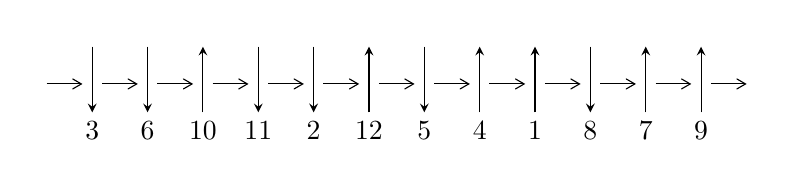
\begin{tikzpicture}[x=20pt, y=17pt]
	% nodes
	\node (C0) at (0, 0) {};
	\node (C1) at (1, 0) {};
	\node (C1U) at (1, +1) {};
	\node (C1D) at (1, -1) {3};

	\node (C2) at (2, 0) {};
	\node (C2U) at (2, +1) {};
	\node (C2D) at (2, -1) {6};

	\node (C3) at (3, 0) {};
	\node (C3U) at (3, +1) {};
	\node (C3D) at (3, -1) {10};

	\node (C4) at (4, 0) {};
	\node (C4U) at (4, +1) {};
	\node (C4D) at (4, -1) {11};

	\node (C5) at (5, 0) {};
	\node (C5U) at (5, +1) {};
	\node (C5D) at (5, -1) {2};

	\node (C6) at (6, 0) {};
	\node (C6U) at (6, +1) {};
	\node (C6D) at (6, -1) {12};

	\node (C7) at (7, 0) {};
	\node (C7U) at (7, +1) {};
	\node (C7D) at (7, -1) {5};

	\node (C8) at (8, 0) {};
	\node (C8U) at (8, +1) {};
	\node (C8D) at (8, -1) {4};

	\node (C9) at (9, 0) {};
	\node (C9U) at (9, +1) {};
	\node (C9D) at (9, -1) {1};

	\node (C10) at (10, 0) {};
	\node (C10U) at (10, +1) {};
	\node (C10D) at (10, -1) {8};

	\node (C11) at (11, 0) {};
	\node (C11U) at (11, +1) {};
	\node (C11D) at (11, -1) {7};

	\node (C12) at (12, 0) {};
	\node (C12U) at (12, +1) {};
	\node (C12D) at (12, -1) {9};
	\node (C13) at (13, 0) {};

	% arrows
	\draw[->,>={angle 60}]
	(C0) edge (C1) (C1) edge (C2) (C2) edge (C3) (C3) edge (C4) (C4) edge (C5) (C5) edge (C6) (C6) edge (C7) (C7) edge (C8) (C8) edge (C9) (C9) edge (C10) (C10) edge (C11) (C11) edge (C12) (C12) edge (C13) ;	\draw[->,>=stealth]
	(C1U) edge (C1D) (C2U) edge (C2D) (C3D) edge (C3U) (C4U) edge (C4D) (C5U) edge (C5D) (C6D) edge (C6U) (C7U) edge (C7D) (C8D) edge (C8U) (C9D) edge (C9U) (C10U) edge (C10D) (C11D) edge (C11U) (C12D) edge (C12U) ;
	\end{tikzpicture} \\
\hhline{~~} \\& 
\textbf{Solving Sequence} \\ \cline{2-2} 
 &
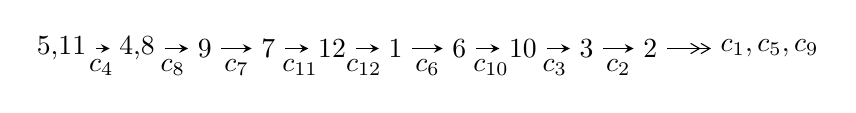
\begin{tikzpicture}[x=23pt, y=7pt]
	% node
	\node (A0) at (-1/8, 0) {5,11};
	\node (A1) at (17/16, 0) {4,8};
	\node (A2) at (17/8, 0) {9};
	\node (A3) at (25/8, 0) {7};
	\node (A4) at (33/8, 0) {12};
	\node (A5) at (41/8, 0) {1};
	\node (A6) at (49/8, 0) {6};
	\node (A7) at (57/8, 0) {10};
	\node (A8) at (65/8, 0) {3};
	\node (A9) at (73/8, 0) {2};
	\node (C1) at (1/2, -1) {$c_{4}$};
	\node (C2) at (13/8, -1) {$c_{8}$};
	\node (C3) at (21/8, -1) {$c_{7}$};
	\node (C4) at (29/8, -1) {$c_{11}$};
	\node (C5) at (37/8, -1) {$c_{12}$};
	\node (C6) at (45/8, -1) {$c_{6}$};
	\node (C7) at (53/8, -1) {$c_{10}$};
	\node (C8) at (61/8, -1) {$c_{3}$};
	\node (C9) at (69/8, -1) {$c_{2}$};
	\node (A10) at (11, 0) {$c_{1},c_{5},c_{9}$};

	% edge
	\draw[->,>=stealth]	
	(A0) edge (A1) (A1) edge (A2) (A2) edge (A3) (A3) edge (A4) (A4) edge (A5) (A5) edge (A6) (A6) edge (A7) (A7) edge (A8) (A8) edge (A9) ;
	\draw[->>,>={angle 60}]	
	(A9) edge (A10);
\end{tikzpicture} \\ 

\end{tabular} \\

\footnotetext{
The image of knot diagram is generated by the software ``\textbf{Draw programme}" developed by Andrew Bartholomew(\url{http://www.layer8.co.uk/maths/draw/index.htm\#Running-draw}), where we modified some parts for our purpose(\url{https://github.com/CATsTAILs/LinksPainter}).
}\phantom \\ \newline 
\centering \textbf{Ideals for irreducible components\footnotemark of $X_{\text{par}}$} 
 
\begin{align*}
I^u_{1}&=\langle 
-1.77444\times10^{1381} u^{163}+2.56374\times10^{1381} u^{162}+\cdots+7.33297\times10^{1381} b+1.54120\times10^{1386},\\
\phantom{I^u_{1}}&\phantom{= \langle  }-1.90440\times10^{1385} u^{163}+2.76814\times10^{1385} u^{162}+\cdots+1.42491\times10^{1386} a+1.59696\times10^{1390},\\
\phantom{I^u_{1}}&\phantom{= \langle  }u^{164}- u^{163}+\cdots-199323 u-38863\rangle \\
I^u_{2}&=\langle 
-1.19980\times10^{32} u^{31}+5.25243\times10^{31} u^{30}+\cdots+7.22842\times10^{32} b+1.39595\times10^{32},\\
\phantom{I^u_{2}}&\phantom{= \langle  }-1.57050\times10^{33} u^{31}+7.88830\times10^{31} u^{30}+\cdots+7.22842\times10^{32} a+5.28812\times10^{32},\;u^{32}-5 u^{30}+\cdots+u^2-1\rangle \\
I^u_{3}&=\langle 
u^2 b+b^2+u^2+2 u+1,\;a,\;u^3+u^2-1\rangle \\
\\
\end{align*}
\raggedright * 3 irreducible components of $\dim_{\mathbb{C}}=0$, with total 202 representations.\\
\footnotetext{All coefficients of polynomials are rational numbers. But the coefficients are sometimes approximated in decimal forms when there is not enough margin.}
\newpage
\renewcommand{\arraystretch}{1}
\centering \section*{I. $I^u_{1}= \langle -1.77\times10^{1381} u^{163}+2.56\times10^{1381} u^{162}+\cdots+7.33\times10^{1381} b+1.54\times10^{1386},\;-1.90\times10^{1385} u^{163}+2.77\times10^{1385} u^{162}+\cdots+1.42\times10^{1386} a+1.60\times10^{1390},\;u^{164}- u^{163}+\cdots-199323 u-38863 \rangle$}
\flushleft \textbf{(i) Arc colorings}\\
\begin{tabular}{m{7pt} m{180pt} m{7pt} m{180pt} }
\flushright $a_{5}=$&$\begin{pmatrix}1\\0\end{pmatrix}$ \\
\flushright $a_{11}=$&$\begin{pmatrix}0\\u\end{pmatrix}$ \\
\flushright $a_{4}=$&$\begin{pmatrix}1\\- u^2\end{pmatrix}$ \\
\flushright $a_{8}=$&$\begin{pmatrix}0.133651 u^{163}-0.194268 u^{162}+\cdots-33659.0 u-11207.4\\0.241981 u^{163}-0.349618 u^{162}+\cdots-60880.2 u-21017.3\end{pmatrix}$ \\
\flushright $a_{9}=$&$\begin{pmatrix}0.402858 u^{163}-0.583065 u^{162}+\cdots-101428. u-34580.5\\0.189046 u^{163}-0.273549 u^{162}+\cdots-47505.5 u-16369.7\end{pmatrix}$ \\
\flushright $a_{7}=$&$\begin{pmatrix}0.375632 u^{163}-0.543886 u^{162}+\cdots-94539.2 u-32224.8\\0.241981 u^{163}-0.349618 u^{162}+\cdots-60880.2 u-21017.3\end{pmatrix}$ \\
\flushright $a_{12}=$&$\begin{pmatrix}0.131044 u^{163}-0.190226 u^{162}+\cdots-33416.6 u-10966.2\\0.207185 u^{163}-0.297226 u^{162}+\cdots-52382.2 u-18227.1\end{pmatrix}$ \\
\flushright $a_{1}=$&$\begin{pmatrix}-0.299579 u^{163}+0.431809 u^{162}+\cdots+75109.5 u+26149.8\\-0.0509614 u^{163}+0.0745900 u^{162}+\cdots+12741.1 u+4334.21\end{pmatrix}$ \\
\flushright $a_{6}=$&$\begin{pmatrix}-0.156762 u^{163}+0.236762 u^{162}+\cdots+38456.7 u+11350.5\\-0.0334928 u^{163}+0.0511943 u^{162}+\cdots+8094.09 u+2542.35\end{pmatrix}$ \\
\flushright $a_{10}=$&$\begin{pmatrix}-0.0723496 u^{163}+0.101726 u^{162}+\cdots+17937.6 u+6889.42\\-0.00379087 u^{163}+0.00527361 u^{162}+\cdots+1030.07 u+371.507\end{pmatrix}$ \\
\flushright $a_{3}=$&$\begin{pmatrix}-0.111960 u^{163}+0.152313 u^{162}+\cdots+27730.2 u+12432.7\\-0.00755907 u^{163}+0.00896551 u^{162}+\cdots+2282.12 u+958.156\end{pmatrix}$ \\
\flushright $a_{2}=$&$\begin{pmatrix}0.264682 u^{163}-0.380139 u^{162}+\cdots-67329.1 u-23429.3\\-0.00515168 u^{163}+0.00983070 u^{162}+\cdots+996.726 u+70.0665\end{pmatrix}$\\&\end{tabular}
\flushleft \textbf{(ii) Obstruction class $= -1$}\\~\\
\flushleft \textbf{(iii) Cusp Shapes $= 1.64850 u^{163}-2.38398 u^{162}+\cdots-416894. u-142792.$}\\~\\
\newpage\renewcommand{\arraystretch}{1}
\flushleft \textbf{(iv) u-Polynomials at the component}\newline \\
\begin{tabular}{m{50pt}|m{274pt}}
Crossings & \hspace{64pt}u-Polynomials at each crossing \\
\hline $$\begin{aligned}c_{1}\end{aligned}$$&$\begin{aligned}
&u^{164}+67 u^{163}+\cdots+5522661 u+35721
\end{aligned}$\\
\hline $$\begin{aligned}c_{2},c_{5}\end{aligned}$$&$\begin{aligned}
&u^{164}+5 u^{163}+\cdots+2781 u+189
\end{aligned}$\\
\hline $$\begin{aligned}c_{3}\end{aligned}$$&$\begin{aligned}
&u^{164}+3 u^{163}+\cdots+905948789 u-782977201
\end{aligned}$\\
\hline $$\begin{aligned}c_{4}\end{aligned}$$&$\begin{aligned}
&u^{164}+u^{163}+\cdots+199323 u-38863
\end{aligned}$\\
\hline $$\begin{aligned}c_{6},c_{11}\end{aligned}$$&$\begin{aligned}
&u^{164}+5 u^{163}+\cdots-10894215 u-899893
\end{aligned}$\\
\hline $$\begin{aligned}c_{7}\end{aligned}$$&$\begin{aligned}
&u^{164}-8 u^{163}+\cdots+35 u-1
\end{aligned}$\\
\hline $$\begin{aligned}c_{8}\end{aligned}$$&$\begin{aligned}
&u^{164}-4 u^{163}+\cdots+38135 u+12557
\end{aligned}$\\
\hline $$\begin{aligned}c_{9},c_{12}\end{aligned}$$&$\begin{aligned}
&u^{164}+3 u^{163}+\cdots-391027 u-16729
\end{aligned}$\\
\hline $$\begin{aligned}c_{10}\end{aligned}$$&$\begin{aligned}
&u^{164}-3 u^{163}+\cdots-6336 u+448
\end{aligned}$\\
\hline
\end{tabular}\\~\\
\newpage\renewcommand{\arraystretch}{1}
\flushleft \textbf{(v) Riley Polynomials at the component}\newline \\
\begin{tabular}{m{50pt}|m{274pt}}
Crossings & \hspace{64pt}Riley Polynomials at each crossing \\
\hline $$\begin{aligned}c_{1}\end{aligned}$$&$\begin{aligned}
&y^{164}+65 y^{163}+\cdots-24187621914549 y+1275989841
\end{aligned}$\\
\hline $$\begin{aligned}c_{2},c_{5}\end{aligned}$$&$\begin{aligned}
&y^{164}-67 y^{163}+\cdots-5522661 y+35721
\end{aligned}$\\
\hline $$\begin{aligned}c_{3}\end{aligned}$$&$\begin{aligned}
&y^{164}-29 y^{163}+\cdots-3.35\times10^{19} y+6.13\times10^{17}
\end{aligned}$\\
\hline $$\begin{aligned}c_{4}\end{aligned}$$&$\begin{aligned}
&y^{164}-39 y^{163}+\cdots-100873049407 y+1510332769
\end{aligned}$\\
\hline $$\begin{aligned}c_{6},c_{11}\end{aligned}$$&$\begin{aligned}
&y^{164}+87 y^{163}+\cdots-44025753748099 y+809807411449
\end{aligned}$\\
\hline $$\begin{aligned}c_{7}\end{aligned}$$&$\begin{aligned}
&y^{164}-20 y^{163}+\cdots-31 y+1
\end{aligned}$\\
\hline $$\begin{aligned}c_{8}\end{aligned}$$&$\begin{aligned}
&y^{164}+4 y^{163}+\cdots-1788168855 y+157678249
\end{aligned}$\\
\hline $$\begin{aligned}c_{9},c_{12}\end{aligned}$$&$\begin{aligned}
&y^{164}-93 y^{163}+\cdots-86202822195 y+279859441
\end{aligned}$\\
\hline $$\begin{aligned}c_{10}\end{aligned}$$&$\begin{aligned}
&y^{164}-5 y^{163}+\cdots+13514752 y+200704
\end{aligned}$\\
\hline
\end{tabular}\\~\\
\newpage\flushleft \textbf{(vi) Complex Volumes and Cusp Shapes}
$$\begin{array}{c|c|c}  
\text{Solutions to }I^u_{1}& \I (\text{vol} + \sqrt{-1}CS) & \text{Cusp shape}\\
 \hline 
\begin{aligned}
u &= \phantom{-}0.680466 + 0.730949 I \\
a &= \phantom{-}1.038340 + 0.087412 I \\
b &= -0.375347 - 0.278447 I\end{aligned}
 & \phantom{-}0.00155 - 2.01871 I & \phantom{-0.000000 } 0 \\ \hline\begin{aligned}
u &= \phantom{-}0.680466 - 0.730949 I \\
a &= \phantom{-}1.038340 - 0.087412 I \\
b &= -0.375347 + 0.278447 I\end{aligned}
 & \phantom{-}0.00155 + 2.01871 I & \phantom{-0.000000 } 0 \\ \hline\begin{aligned}
u &= \phantom{-}0.927280 + 0.387187 I \\
a &= -0.601355 + 0.229591 I \\
b &= \phantom{-}0.836521 + 0.938576 I\end{aligned}
 & -1.78213 - 2.95331 I & \phantom{-0.000000 } 0 \\ \hline\begin{aligned}
u &= \phantom{-}0.927280 - 0.387187 I \\
a &= -0.601355 - 0.229591 I \\
b &= \phantom{-}0.836521 - 0.938576 I\end{aligned}
 & -1.78213 + 2.95331 I & \phantom{-0.000000 } 0 \\ \hline\begin{aligned}
u &= -0.843599 + 0.517527 I \\
a &= -1.387700 + 0.216491 I \\
b &= \phantom{-}0.982676 - 0.446845 I\end{aligned}
 & -3.09467 + 3.85973 I & \phantom{-0.000000 } 0 \\ \hline\begin{aligned}
u &= -0.843599 - 0.517527 I \\
a &= -1.387700 - 0.216491 I \\
b &= \phantom{-}0.982676 + 0.446845 I\end{aligned}
 & -3.09467 - 3.85973 I & \phantom{-0.000000 } 0 \\ \hline\begin{aligned}
u &= -0.851750 + 0.485246 I \\
a &= \phantom{-}0.509555 - 0.020321 I \\
b &= -1.17275 + 1.03663 I\end{aligned}
 & -4.78088 - 0.83728 I & \phantom{-0.000000 } 0 \\ \hline\begin{aligned}
u &= -0.851750 - 0.485246 I \\
a &= \phantom{-}0.509555 + 0.020321 I \\
b &= -1.17275 - 1.03663 I\end{aligned}
 & -4.78088 + 0.83728 I & \phantom{-0.000000 } 0 \\ \hline\begin{aligned}
u &= -0.299506 + 1.009890 I \\
a &= \phantom{-}0.733451 - 0.344211 I \\
b &= \phantom{-}0.156881 + 0.519142 I\end{aligned}
 & \phantom{-}1.22207 - 1.56871 I & \phantom{-0.000000 } 0 \\ \hline\begin{aligned}
u &= -0.299506 - 1.009890 I \\
a &= \phantom{-}0.733451 + 0.344211 I \\
b &= \phantom{-}0.156881 - 0.519142 I\end{aligned}
 & \phantom{-}1.22207 + 1.56871 I & \phantom{-0.000000 } 0\\
 \hline 
 \end{array}$$\newpage$$\begin{array}{c|c|c}  
\text{Solutions to }I^u_{1}& \I (\text{vol} + \sqrt{-1}CS) & \text{Cusp shape}\\
 \hline 
\begin{aligned}
u &= \phantom{-}0.545812 + 0.920218 I \\
a &= \phantom{-}0.596485 + 0.246527 I \\
b &= -1.41923 - 1.18093 I\end{aligned}
 & \phantom{-}2.79343 - 10.68100 I & \phantom{-0.000000 } 0 \\ \hline\begin{aligned}
u &= \phantom{-}0.545812 - 0.920218 I \\
a &= \phantom{-}0.596485 - 0.246527 I \\
b &= -1.41923 + 1.18093 I\end{aligned}
 & \phantom{-}2.79343 + 10.68100 I & \phantom{-0.000000 } 0 \\ \hline\begin{aligned}
u &= \phantom{-}0.774452 + 0.740437 I \\
a &= -1.031990 + 0.114079 I \\
b &= \phantom{-}1.55469 + 0.14991 I\end{aligned}
 & \phantom{-}1.74329 - 8.48712 I & \phantom{-0.000000 } 0 \\ \hline\begin{aligned}
u &= \phantom{-}0.774452 - 0.740437 I \\
a &= -1.031990 - 0.114079 I \\
b &= \phantom{-}1.55469 - 0.14991 I\end{aligned}
 & \phantom{-}1.74329 + 8.48712 I & \phantom{-0.000000 } 0 \\ \hline\begin{aligned}
u &= \phantom{-}0.743875 + 0.773402 I \\
a &= -0.505902 - 0.339116 I \\
b &= \phantom{-}0.298426 + 1.096570 I\end{aligned}
 & \phantom{-}2.57813 - 2.81733 I & \phantom{-0.000000 } 0 \\ \hline\begin{aligned}
u &= \phantom{-}0.743875 - 0.773402 I \\
a &= -0.505902 + 0.339116 I \\
b &= \phantom{-}0.298426 - 1.096570 I\end{aligned}
 & \phantom{-}2.57813 + 2.81733 I & \phantom{-0.000000 } 0 \\ \hline\begin{aligned}
u &= -0.853525 + 0.355800 I \\
a &= \phantom{-}0.523747 + 1.227710 I \\
b &= -0.779577 + 0.425320 I\end{aligned}
 & -6.23476 + 5.13208 I & \phantom{-0.000000 } 0 \\ \hline\begin{aligned}
u &= -0.853525 - 0.355800 I \\
a &= \phantom{-}0.523747 - 1.227710 I \\
b &= -0.779577 - 0.425320 I\end{aligned}
 & -6.23476 - 5.13208 I & \phantom{-0.000000 } 0 \\ \hline\begin{aligned}
u &= \phantom{-}0.875599 + 0.271069 I \\
a &= -1.38289 + 1.04344 I \\
b &= \phantom{-}1.124580 + 0.517580 I\end{aligned}
 & \phantom{-}0.33289 - 5.96595 I & \phantom{-0.000000 } 0 \\ \hline\begin{aligned}
u &= \phantom{-}0.875599 - 0.271069 I \\
a &= -1.38289 - 1.04344 I \\
b &= \phantom{-}1.124580 - 0.517580 I\end{aligned}
 & \phantom{-}0.33289 + 5.96595 I & \phantom{-0.000000 } 0\\
 \hline 
 \end{array}$$\newpage$$\begin{array}{c|c|c}  
\text{Solutions to }I^u_{1}& \I (\text{vol} + \sqrt{-1}CS) & \text{Cusp shape}\\
 \hline 
\begin{aligned}
u &= \phantom{-}0.874528 + 0.252780 I \\
a &= \phantom{-}0.563408 + 0.009092 I \\
b &= -0.517700 + 1.243300 I\end{aligned}
 & -2.00026 - 4.44909 I & \phantom{-0.000000 } 0 \\ \hline\begin{aligned}
u &= \phantom{-}0.874528 - 0.252780 I \\
a &= \phantom{-}0.563408 - 0.009092 I \\
b &= -0.517700 - 1.243300 I\end{aligned}
 & -2.00026 + 4.44909 I & \phantom{-0.000000 } 0 \\ \hline\begin{aligned}
u &= \phantom{-}0.846044 + 0.309569 I \\
a &= -0.044037 - 0.250058 I \\
b &= \phantom{-}0.31737 + 1.80080 I\end{aligned}
 & -2.89263 - 1.61904 I & \phantom{-0.000000 } 0 \\ \hline\begin{aligned}
u &= \phantom{-}0.846044 - 0.309569 I \\
a &= -0.044037 + 0.250058 I \\
b &= \phantom{-}0.31737 - 1.80080 I\end{aligned}
 & -2.89263 + 1.61904 I & \phantom{-0.000000 } 0 \\ \hline\begin{aligned}
u &= -0.693945 + 0.558606 I \\
a &= \phantom{-}0.85689 + 1.26010 I \\
b &= -0.626254 + 0.087986 I\end{aligned}
 & \phantom{-}2.64856 + 0.63147 I & \phantom{-0.000000 } 0 \\ \hline\begin{aligned}
u &= -0.693945 - 0.558606 I \\
a &= \phantom{-}0.85689 - 1.26010 I \\
b &= -0.626254 - 0.087986 I\end{aligned}
 & \phantom{-}2.64856 - 0.63147 I & \phantom{-0.000000 } 0 \\ \hline\begin{aligned}
u &= \phantom{-}0.867258 + 0.188145 I \\
a &= \phantom{-}0.98669 - 1.35007 I \\
b &= -0.988365 - 0.156922 I\end{aligned}
 & -7.27121 + 0.84000 I & \phantom{-0.000000 } 0 \\ \hline\begin{aligned}
u &= \phantom{-}0.867258 - 0.188145 I \\
a &= \phantom{-}0.98669 + 1.35007 I \\
b &= -0.988365 + 0.156922 I\end{aligned}
 & -7.27121 - 0.84000 I & \phantom{-0.000000 } 0 \\ \hline\begin{aligned}
u &= -0.846508 + 0.265557 I \\
a &= \phantom{-}1.45793 + 1.33875 I \\
b &= -1.138390 + 0.406086 I\end{aligned}
 & -0.99704 + 11.80640 I & \phantom{-0.000000 } 0 \\ \hline\begin{aligned}
u &= -0.846508 - 0.265557 I \\
a &= \phantom{-}1.45793 - 1.33875 I \\
b &= -1.138390 - 0.406086 I\end{aligned}
 & -0.99704 - 11.80640 I & \phantom{-0.000000 } 0\\
 \hline 
 \end{array}$$\newpage$$\begin{array}{c|c|c}  
\text{Solutions to }I^u_{1}& \I (\text{vol} + \sqrt{-1}CS) & \text{Cusp shape}\\
 \hline 
\begin{aligned}
u &= -0.698209 + 0.871774 I \\
a &= \phantom{-}0.372443 - 0.378178 I \\
b &= -0.028536 + 1.048580 I\end{aligned}
 & \phantom{-}2.33040 - 2.22642 I & \phantom{-0.000000 } 0 \\ \hline\begin{aligned}
u &= -0.698209 - 0.871774 I \\
a &= \phantom{-}0.372443 + 0.378178 I \\
b &= -0.028536 - 1.048580 I\end{aligned}
 & \phantom{-}2.33040 + 2.22642 I & \phantom{-0.000000 } 0 \\ \hline\begin{aligned}
u &= -0.818604 + 0.329022 I \\
a &= \phantom{-}0.282166 - 0.249552 I \\
b &= -0.75275 + 1.81617 I\end{aligned}
 & -3.76321 + 5.76423 I & \phantom{-0.000000 } 0 \\ \hline\begin{aligned}
u &= -0.818604 - 0.329022 I \\
a &= \phantom{-}0.282166 + 0.249552 I \\
b &= -0.75275 - 1.81617 I\end{aligned}
 & -3.76321 - 5.76423 I & \phantom{-0.000000 } 0 \\ \hline\begin{aligned}
u &= -0.802770 + 0.793673 I \\
a &= -0.814488 + 0.547392 I \\
b &= -0.158402 + 0.074439 I\end{aligned}
 & -2.63474 - 1.83561 I & \phantom{-0.000000 } 0 \\ \hline\begin{aligned}
u &= -0.802770 - 0.793673 I \\
a &= -0.814488 - 0.547392 I \\
b &= -0.158402 - 0.074439 I\end{aligned}
 & -2.63474 + 1.83561 I & \phantom{-0.000000 } 0 \\ \hline\begin{aligned}
u &= -0.656043 + 0.566699 I \\
a &= \phantom{-}1.79126 - 0.68503 I \\
b &= -0.582715 + 0.987299 I\end{aligned}
 & \phantom{-}5.88468 - 3.09996 I & \phantom{-0.000000 } 0 \\ \hline\begin{aligned}
u &= -0.656043 - 0.566699 I \\
a &= \phantom{-}1.79126 + 0.68503 I \\
b &= -0.582715 - 0.987299 I\end{aligned}
 & \phantom{-}5.88468 + 3.09996 I & \phantom{-0.000000 } 0 \\ \hline\begin{aligned}
u &= -0.865508\phantom{ +0.000000I} \\
a &= \phantom{-}0.998864\phantom{ +0.000000I} \\
b &= -0.360743\phantom{ +0.000000I}\end{aligned}
 & \phantom{-}1.96171\phantom{ +0.000000I} & \phantom{-0.000000 } 0 \\ \hline\begin{aligned}
u &= -0.835896 + 0.779708 I \\
a &= \phantom{-}1.134000 + 0.039294 I \\
b &= -1.62721 + 0.56445 I\end{aligned}
 & \phantom{-}2.89514 + 4.46818 I & \phantom{-0.000000 } 0\\
 \hline 
 \end{array}$$\newpage$$\begin{array}{c|c|c}  
\text{Solutions to }I^u_{1}& \I (\text{vol} + \sqrt{-1}CS) & \text{Cusp shape}\\
 \hline 
\begin{aligned}
u &= -0.835896 - 0.779708 I \\
a &= \phantom{-}1.134000 - 0.039294 I \\
b &= -1.62721 - 0.56445 I\end{aligned}
 & \phantom{-}2.89514 - 4.46818 I & \phantom{-0.000000 } 0 \\ \hline\begin{aligned}
u &= \phantom{-}0.592169 + 0.618906 I \\
a &= -1.00822 + 1.45400 I \\
b &= \phantom{-}0.647819 + 0.273580 I\end{aligned}
 & \phantom{-}1.82269 + 3.88071 I & \phantom{-0.000000 } 0 \\ \hline\begin{aligned}
u &= \phantom{-}0.592169 - 0.618906 I \\
a &= -1.00822 - 1.45400 I \\
b &= \phantom{-}0.647819 - 0.273580 I\end{aligned}
 & \phantom{-}1.82269 - 3.88071 I & \phantom{-0.000000 } 0 \\ \hline\begin{aligned}
u &= -0.822787 + 0.186849 I \\
a &= -0.989797 + 0.216146 I \\
b &= \phantom{-}0.855341 + 0.843210 I\end{aligned}
 & -1.97814 - 0.47061 I & \phantom{-0.000000 } 0 \\ \hline\begin{aligned}
u &= -0.822787 - 0.186849 I \\
a &= -0.989797 - 0.216146 I \\
b &= \phantom{-}0.855341 - 0.843210 I\end{aligned}
 & -1.97814 + 0.47061 I & \phantom{-0.000000 } 0 \\ \hline\begin{aligned}
u &= \phantom{-}0.257378 + 0.790500 I \\
a &= \phantom{-}1.039660 + 0.344122 I \\
b &= -0.517493 - 1.118250 I\end{aligned}
 & \phantom{-}7.67892 - 0.09577 I & \phantom{-0.000000 } 0 \\ \hline\begin{aligned}
u &= \phantom{-}0.257378 - 0.790500 I \\
a &= \phantom{-}1.039660 - 0.344122 I \\
b &= -0.517493 + 1.118250 I\end{aligned}
 & \phantom{-}7.67892 + 0.09577 I & \phantom{-0.000000 } 0 \\ \hline\begin{aligned}
u &= \phantom{-}0.907691 + 0.737628 I \\
a &= \phantom{-}1.223800 + 0.443783 I \\
b &= -0.497324 - 0.885819 I\end{aligned}
 & \phantom{-}2.12353 - 2.79649 I & \phantom{-0.000000 } 0 \\ \hline\begin{aligned}
u &= \phantom{-}0.907691 - 0.737628 I \\
a &= \phantom{-}1.223800 - 0.443783 I \\
b &= -0.497324 + 0.885819 I\end{aligned}
 & \phantom{-}2.12353 + 2.79649 I & \phantom{-0.000000 } 0 \\ \hline\begin{aligned}
u &= \phantom{-}0.664275 + 0.483548 I \\
a &= -1.96988 - 0.76374 I \\
b &= \phantom{-}0.774716 + 0.908547 I\end{aligned}
 & \phantom{-}6.18139 - 2.62276 I & \phantom{-0.000000 } 0\\
 \hline 
 \end{array}$$\newpage$$\begin{array}{c|c|c}  
\text{Solutions to }I^u_{1}& \I (\text{vol} + \sqrt{-1}CS) & \text{Cusp shape}\\
 \hline 
\begin{aligned}
u &= \phantom{-}0.664275 - 0.483548 I \\
a &= -1.96988 + 0.76374 I \\
b &= \phantom{-}0.774716 - 0.908547 I\end{aligned}
 & \phantom{-}6.18139 + 2.62276 I & \phantom{-0.000000 } 0 \\ \hline\begin{aligned}
u &= -0.939376 + 0.727530 I \\
a &= -0.122764 + 0.961920 I \\
b &= -0.468747 - 0.434483 I\end{aligned}
 & \phantom{-}3.83500 - 1.56652 I & \phantom{-0.000000 } 0 \\ \hline\begin{aligned}
u &= -0.939376 - 0.727530 I \\
a &= -0.122764 - 0.961920 I \\
b &= -0.468747 + 0.434483 I\end{aligned}
 & \phantom{-}3.83500 + 1.56652 I & \phantom{-0.000000 } 0 \\ \hline\begin{aligned}
u &= -0.883077 + 0.803222 I \\
a &= \phantom{-}1.156990 - 0.114025 I \\
b &= -1.51485 + 1.07417 I\end{aligned}
 & \phantom{-}4.00763 + 7.44935 I & \phantom{-0.000000 } 0 \\ \hline\begin{aligned}
u &= -0.883077 - 0.803222 I \\
a &= \phantom{-}1.156990 + 0.114025 I \\
b &= -1.51485 - 1.07417 I\end{aligned}
 & \phantom{-}4.00763 - 7.44935 I & \phantom{-0.000000 } 0 \\ \hline\begin{aligned}
u &= -0.953787 + 0.727406 I \\
a &= -1.293840 + 0.413643 I \\
b &= \phantom{-}0.640840 - 0.982440 I\end{aligned}
 & \phantom{-}1.51782 + 8.04547 I & \phantom{-0.000000 } 0 \\ \hline\begin{aligned}
u &= -0.953787 - 0.727406 I \\
a &= -1.293840 - 0.413643 I \\
b &= \phantom{-}0.640840 + 0.982440 I\end{aligned}
 & \phantom{-}1.51782 - 8.04547 I & \phantom{-0.000000 } 0 \\ \hline\begin{aligned}
u &= \phantom{-}0.761351 + 0.234087 I \\
a &= \phantom{-}1.65530 - 1.56070 I \\
b &= -1.326950 - 0.062869 I\end{aligned}
 & -4.39098 - 4.83003 I & \phantom{-0.000000 } 0 \\ \hline\begin{aligned}
u &= \phantom{-}0.761351 - 0.234087 I \\
a &= \phantom{-}1.65530 + 1.56070 I \\
b &= -1.326950 + 0.062869 I\end{aligned}
 & -4.39098 + 4.83003 I & \phantom{-0.000000 } 0 \\ \hline\begin{aligned}
u &= -0.303472 + 0.730608 I \\
a &= \phantom{-}0.944158 + 0.091808 I \\
b &= -0.095955 + 0.568295 I\end{aligned}
 & \phantom{-}1.30056 - 0.86249 I & \phantom{-0.000000 } 0\\
 \hline 
 \end{array}$$\newpage$$\begin{array}{c|c|c}  
\text{Solutions to }I^u_{1}& \I (\text{vol} + \sqrt{-1}CS) & \text{Cusp shape}\\
 \hline 
\begin{aligned}
u &= -0.303472 - 0.730608 I \\
a &= \phantom{-}0.944158 - 0.091808 I \\
b &= -0.095955 - 0.568295 I\end{aligned}
 & \phantom{-}1.30056 + 0.86249 I & \phantom{-0.000000 } 0 \\ \hline\begin{aligned}
u &= \phantom{-}0.894889 + 0.812960 I \\
a &= -1.090370 - 0.156839 I \\
b &= \phantom{-}1.32567 + 1.17013 I\end{aligned}
 & \phantom{-}3.88431 - 2.58081 I & \phantom{-0.000000 } 0 \\ \hline\begin{aligned}
u &= \phantom{-}0.894889 - 0.812960 I \\
a &= -1.090370 + 0.156839 I \\
b &= \phantom{-}1.32567 - 1.17013 I\end{aligned}
 & \phantom{-}3.88431 + 2.58081 I & \phantom{-0.000000 } 0 \\ \hline\begin{aligned}
u &= -0.724161 + 0.283539 I \\
a &= -1.61444 - 0.52551 I \\
b &= \phantom{-}2.04433 - 0.51453 I\end{aligned}
 & -3.36554 + 1.98527 I & \phantom{-0.000000 } 0 \\ \hline\begin{aligned}
u &= -0.724161 - 0.283539 I \\
a &= -1.61444 + 0.52551 I \\
b &= \phantom{-}2.04433 + 0.51453 I\end{aligned}
 & -3.36554 - 1.98527 I & \phantom{-0.000000 } 0 \\ \hline\begin{aligned}
u &= -0.744608 + 0.212748 I \\
a &= -1.79424 - 1.20517 I \\
b &= \phantom{-}1.47956 - 0.15655 I\end{aligned}
 & -3.45898 + 0.01298 I & \phantom{-0.000000 } 0 \\ \hline\begin{aligned}
u &= -0.744608 - 0.212748 I \\
a &= -1.79424 + 1.20517 I \\
b &= \phantom{-}1.47956 + 0.15655 I\end{aligned}
 & -3.45898 - 0.01298 I & \phantom{-0.000000 } 0 \\ \hline\begin{aligned}
u &= \phantom{-}0.938831 + 0.788723 I \\
a &= \phantom{-}0.381007 + 0.844548 I \\
b &= \phantom{-}0.332972 - 0.547804 I\end{aligned}
 & \phantom{-}3.77456 - 3.46134 I & \phantom{-0.000000 } 0 \\ \hline\begin{aligned}
u &= \phantom{-}0.938831 - 0.788723 I \\
a &= \phantom{-}0.381007 - 0.844548 I \\
b &= \phantom{-}0.332972 + 0.547804 I\end{aligned}
 & \phantom{-}3.77456 + 3.46134 I & \phantom{-0.000000 } 0 \\ \hline\begin{aligned}
u &= -0.721359 + 0.991652 I \\
a &= \phantom{-}0.910790 - 0.090767 I \\
b &= -0.751303 + 0.186959 I\end{aligned}
 & \phantom{-}4.33020 + 4.68324 I & \phantom{-0.000000 } 0\\
 \hline 
 \end{array}$$\newpage$$\begin{array}{c|c|c}  
\text{Solutions to }I^u_{1}& \I (\text{vol} + \sqrt{-1}CS) & \text{Cusp shape}\\
 \hline 
\begin{aligned}
u &= -0.721359 - 0.991652 I \\
a &= \phantom{-}0.910790 + 0.090767 I \\
b &= -0.751303 - 0.186959 I\end{aligned}
 & \phantom{-}4.33020 - 4.68324 I & \phantom{-0.000000 } 0 \\ \hline\begin{aligned}
u &= -0.585247 + 1.079620 I \\
a &= -0.496503 + 0.241830 I \\
b &= \phantom{-}1.17138 - 0.98304 I\end{aligned}
 & \phantom{-}4.75759 + 4.36318 I & \phantom{-0.000000 } 0 \\ \hline\begin{aligned}
u &= -0.585247 - 1.079620 I \\
a &= -0.496503 - 0.241830 I \\
b &= \phantom{-}1.17138 + 0.98304 I\end{aligned}
 & \phantom{-}4.75759 - 4.36318 I & \phantom{-0.000000 } 0 \\ \hline\begin{aligned}
u &= \phantom{-}0.697062 + 0.316494 I \\
a &= \phantom{-}1.50497 - 0.44251 I \\
b &= -2.17681 - 0.74965 I\end{aligned}
 & -4.10661 + 2.57768 I & \phantom{-0.000000 } 0 \\ \hline\begin{aligned}
u &= \phantom{-}0.697062 - 0.316494 I \\
a &= \phantom{-}1.50497 + 0.44251 I \\
b &= -2.17681 + 0.74965 I\end{aligned}
 & -4.10661 - 2.57768 I & \phantom{-0.000000 } 0 \\ \hline\begin{aligned}
u &= \phantom{-}0.855313 + 0.904264 I \\
a &= -1.360610 - 0.104658 I \\
b &= \phantom{-}0.609321 + 0.935027 I\end{aligned}
 & \phantom{-}5.2831 - 13.6138 I & \phantom{-0.000000 } 0 \\ \hline\begin{aligned}
u &= \phantom{-}0.855313 - 0.904264 I \\
a &= -1.360610 + 0.104658 I \\
b &= \phantom{-}0.609321 - 0.935027 I\end{aligned}
 & \phantom{-}5.2831 + 13.6138 I & \phantom{-0.000000 } 0 \\ \hline\begin{aligned}
u &= -0.348770 + 0.668497 I \\
a &= -1.193380 + 0.399575 I \\
b &= \phantom{-}0.585447 - 1.273580 I\end{aligned}
 & \phantom{-}6.46899 + 6.24386 I & \phantom{-0.000000 } 0 \\ \hline\begin{aligned}
u &= -0.348770 - 0.668497 I \\
a &= -1.193380 - 0.399575 I \\
b &= \phantom{-}0.585447 + 1.273580 I\end{aligned}
 & \phantom{-}6.46899 - 6.24386 I & \phantom{-0.000000 } 0 \\ \hline\begin{aligned}
u &= -0.865030 + 0.908979 I \\
a &= \phantom{-}1.281090 - 0.174043 I \\
b &= -0.588525 + 0.844776 I\end{aligned}
 & \phantom{-}6.69889 + 7.89913 I & \phantom{-0.000000 } 0\\
 \hline 
 \end{array}$$\newpage$$\begin{array}{c|c|c}  
\text{Solutions to }I^u_{1}& \I (\text{vol} + \sqrt{-1}CS) & \text{Cusp shape}\\
 \hline 
\begin{aligned}
u &= -0.865030 - 0.908979 I \\
a &= \phantom{-}1.281090 + 0.174043 I \\
b &= -0.588525 - 0.844776 I\end{aligned}
 & \phantom{-}6.69889 - 7.89913 I & \phantom{-0.000000 } 0 \\ \hline\begin{aligned}
u &= \phantom{-}0.869545 + 0.907139 I \\
a &= -1.112880 + 0.003078 I \\
b &= \phantom{-}0.885115 + 0.882194 I\end{aligned}
 & \phantom{-}0.56042 - 7.08818 I & \phantom{-0.000000 } 0 \\ \hline\begin{aligned}
u &= \phantom{-}0.869545 - 0.907139 I \\
a &= -1.112880 - 0.003078 I \\
b &= \phantom{-}0.885115 - 0.882194 I\end{aligned}
 & \phantom{-}0.56042 + 7.08818 I & \phantom{-0.000000 } 0 \\ \hline\begin{aligned}
u &= \phantom{-}0.335556 + 0.655229 I \\
a &= -0.875491 + 0.039648 I \\
b &= \phantom{-}1.110760 - 0.594061 I\end{aligned}
 & -0.225668 - 0.934094 I & \phantom{-0.000000 } 0 \\ \hline\begin{aligned}
u &= \phantom{-}0.335556 - 0.655229 I \\
a &= -0.875491 - 0.039648 I \\
b &= \phantom{-}1.110760 + 0.594061 I\end{aligned}
 & -0.225668 + 0.934094 I & \phantom{-0.000000 } 0 \\ \hline\begin{aligned}
u &= \phantom{-}0.410318 + 1.195580 I \\
a &= -0.581246 - 0.466023 I \\
b &= -0.365149 + 0.473190 I\end{aligned}
 & -0.64204 + 6.58118 I & \phantom{-0.000000 } 0 \\ \hline\begin{aligned}
u &= \phantom{-}0.410318 - 1.195580 I \\
a &= -0.581246 + 0.466023 I \\
b &= -0.365149 - 0.473190 I\end{aligned}
 & -0.64204 - 6.58118 I & \phantom{-0.000000 } 0 \\ \hline\begin{aligned}
u &= \phantom{-}0.241740 + 0.660199 I \\
a &= \phantom{-}1.81277 - 1.64202 I \\
b &= \phantom{-}0.012805 - 0.214962 I\end{aligned}
 & -0.91722 - 1.51438 I & \phantom{-0.000000 } 0 \\ \hline\begin{aligned}
u &= \phantom{-}0.241740 - 0.660199 I \\
a &= \phantom{-}1.81277 + 1.64202 I \\
b &= \phantom{-}0.012805 + 0.214962 I\end{aligned}
 & -0.91722 + 1.51438 I & \phantom{-0.000000 } 0 \\ \hline\begin{aligned}
u &= -0.686271 + 0.135352 I \\
a &= -1.34772 - 0.94152 I \\
b &= \phantom{-}1.247450 - 0.663014 I\end{aligned}
 & -3.79316 + 0.49402 I & \phantom{-0.000000 } 0\\
 \hline 
 \end{array}$$\newpage$$\begin{array}{c|c|c}  
\text{Solutions to }I^u_{1}& \I (\text{vol} + \sqrt{-1}CS) & \text{Cusp shape}\\
 \hline 
\begin{aligned}
u &= -0.686271 - 0.135352 I \\
a &= -1.34772 + 0.94152 I \\
b &= \phantom{-}1.247450 + 0.663014 I\end{aligned}
 & -3.79316 - 0.49402 I & \phantom{-0.000000 } 0 \\ \hline\begin{aligned}
u &= \phantom{-}0.298237 + 0.578852 I \\
a &= -1.38184 + 1.93644 I \\
b &= \phantom{-}0.306882 + 0.428918 I\end{aligned}
 & \phantom{-}0.196469 - 1.352020 I & \phantom{-0.000000 } 0 \\ \hline\begin{aligned}
u &= \phantom{-}0.298237 - 0.578852 I \\
a &= -1.38184 - 1.93644 I \\
b &= \phantom{-}0.306882 - 0.428918 I\end{aligned}
 & \phantom{-}0.196469 + 1.352020 I & \phantom{-0.000000 } 0 \\ \hline\begin{aligned}
u &= \phantom{-}0.563884 + 0.293134 I \\
a &= \phantom{-}1.121540 - 0.531986 I \\
b &= -1.83087 - 1.27408 I\end{aligned}
 & -5.93828 - 2.88611 I & \phantom{-0.000000 } 0 \\ \hline\begin{aligned}
u &= \phantom{-}0.563884 - 0.293134 I \\
a &= \phantom{-}1.121540 + 0.531986 I \\
b &= -1.83087 + 1.27408 I\end{aligned}
 & -5.93828 + 2.88611 I & \phantom{-0.000000 } 0 \\ \hline\begin{aligned}
u &= \phantom{-}0.618539\phantom{ +0.000000I} \\
a &= -0.417565\phantom{ +0.000000I} \\
b &= \phantom{-}0.688252\phantom{ +0.000000I}\end{aligned}
 & -1.46636\phantom{ +0.000000I} & \phantom{-0.000000 } 0 \\ \hline\begin{aligned}
u &= \phantom{-}1.175570 + 0.728537 I \\
a &= -0.670080 - 0.066297 I \\
b &= \phantom{-}0.884233 + 0.993981 I\end{aligned}
 & -1.63476 - 3.53703 I & \phantom{-0.000000 } 0 \\ \hline\begin{aligned}
u &= \phantom{-}1.175570 - 0.728537 I \\
a &= -0.670080 + 0.066297 I \\
b &= \phantom{-}0.884233 - 0.993981 I\end{aligned}
 & -1.63476 + 3.53703 I & \phantom{-0.000000 } 0 \\ \hline\begin{aligned}
u &= \phantom{-}1.394300 + 0.001986 I \\
a &= -0.299484 - 0.835963 I \\
b &= \phantom{-}0.35768 + 1.49140 I\end{aligned}
 & \phantom{-}4.15799 - 0.36011 I & \phantom{-0.000000 } 0 \\ \hline\begin{aligned}
u &= \phantom{-}1.394300 - 0.001986 I \\
a &= -0.299484 + 0.835963 I \\
b &= \phantom{-}0.35768 - 1.49140 I\end{aligned}
 & \phantom{-}4.15799 + 0.36011 I & \phantom{-0.000000 } 0\\
 \hline 
 \end{array}$$\newpage$$\begin{array}{c|c|c}  
\text{Solutions to }I^u_{1}& \I (\text{vol} + \sqrt{-1}CS) & \text{Cusp shape}\\
 \hline 
\begin{aligned}
u &= -1.395650 + 0.154090 I \\
a &= -0.004097 + 0.902970 I \\
b &= -0.07106 - 1.55279 I\end{aligned}
 & \phantom{-}3.95984 + 6.13218 I & \phantom{-0.000000 } 0 \\ \hline\begin{aligned}
u &= -1.395650 - 0.154090 I \\
a &= -0.004097 - 0.902970 I \\
b &= -0.07106 + 1.55279 I\end{aligned}
 & \phantom{-}3.95984 - 6.13218 I & \phantom{-0.000000 } 0 \\ \hline\begin{aligned}
u &= -0.588280 + 0.013423 I \\
a &= \phantom{-}1.50174 + 0.67687 I \\
b &= -1.93868 + 1.15727 I\end{aligned}
 & \phantom{-}0.08821 - 10.56030 I & \phantom{-0.000000 } 0 \\ \hline\begin{aligned}
u &= -0.588280 - 0.013423 I \\
a &= \phantom{-}1.50174 - 0.67687 I \\
b &= -1.93868 - 1.15727 I\end{aligned}
 & \phantom{-}0.08821 + 10.56030 I & \phantom{-0.000000 } 0 \\ \hline\begin{aligned}
u &= \phantom{-}0.572181 + 0.026494 I \\
a &= -1.57963 - 0.91589 I \\
b &= \phantom{-}1.70848 - 0.96450 I\end{aligned}
 & \phantom{-}1.66279 - 4.87054 I & \phantom{-0.000000 } 0 \\ \hline\begin{aligned}
u &= \phantom{-}0.572181 - 0.026494 I \\
a &= -1.57963 + 0.91589 I \\
b &= \phantom{-}1.70848 + 0.96450 I\end{aligned}
 & \phantom{-}1.66279 + 4.87054 I & \phantom{-0.000000 } 0 \\ \hline\begin{aligned}
u &= \phantom{-}1.20362 + 0.82210 I \\
a &= \phantom{-}1.055130 + 0.297394 I \\
b &= -1.28769 - 1.27485 I\end{aligned}
 & -2.91003 - 13.62930 I & \phantom{-0.000000 } 0 \\ \hline\begin{aligned}
u &= \phantom{-}1.20362 - 0.82210 I \\
a &= \phantom{-}1.055130 - 0.297394 I \\
b &= -1.28769 + 1.27485 I\end{aligned}
 & -2.91003 + 13.62930 I & \phantom{-0.000000 } 0 \\ \hline\begin{aligned}
u &= -1.22695 + 0.79303 I \\
a &= -0.996786 + 0.347190 I \\
b &= \phantom{-}1.15835 - 1.27098 I\end{aligned}
 & -1.37089 + 8.22540 I & \phantom{-0.000000 } 0 \\ \hline\begin{aligned}
u &= -1.22695 - 0.79303 I \\
a &= -0.996786 - 0.347190 I \\
b &= \phantom{-}1.15835 + 1.27098 I\end{aligned}
 & -1.37089 - 8.22540 I & \phantom{-0.000000 } 0\\
 \hline 
 \end{array}$$\newpage$$\begin{array}{c|c|c}  
\text{Solutions to }I^u_{1}& \I (\text{vol} + \sqrt{-1}CS) & \text{Cusp shape}\\
 \hline 
\begin{aligned}
u &= \phantom{-}1.18536 + 0.87177 I \\
a &= \phantom{-}0.047675 + 0.415271 I \\
b &= \phantom{-}0.158341 - 1.058200 I\end{aligned}
 & \phantom{-}4.50770 + 6.95688 I & \phantom{-0.000000 } 0 \\ \hline\begin{aligned}
u &= \phantom{-}1.18536 - 0.87177 I \\
a &= \phantom{-}0.047675 - 0.415271 I \\
b &= \phantom{-}0.158341 + 1.058200 I\end{aligned}
 & \phantom{-}4.50770 - 6.95688 I & \phantom{-0.000000 } 0 \\ \hline\begin{aligned}
u &= -1.17909 + 0.88109 I \\
a &= \phantom{-}0.672968 + 0.036672 I \\
b &= -0.972213 + 0.986147 I\end{aligned}
 & -4.92183 + 8.27385 I & \phantom{-0.000000 } 0 \\ \hline\begin{aligned}
u &= -1.17909 - 0.88109 I \\
a &= \phantom{-}0.672968 - 0.036672 I \\
b &= -0.972213 - 0.986147 I\end{aligned}
 & -4.92183 - 8.27385 I & \phantom{-0.000000 } 0 \\ \hline\begin{aligned}
u &= -0.398326 + 0.298642 I \\
a &= -1.58795 - 0.49709 I \\
b &= \phantom{-}0.573121 + 0.525290 I\end{aligned}
 & -2.00017 - 1.11829 I & \phantom{-0.000000 } 0 \\ \hline\begin{aligned}
u &= -0.398326 - 0.298642 I \\
a &= -1.58795 + 0.49709 I \\
b &= \phantom{-}0.573121 - 0.525290 I\end{aligned}
 & -2.00017 + 1.11829 I & \phantom{-0.000000 } 0 \\ \hline\begin{aligned}
u &= -1.15338 + 0.98412 I \\
a &= -0.136239 + 0.369762 I \\
b &= \phantom{-}0.079148 - 1.000720 I\end{aligned}
 & \phantom{-}6.03588 - 1.06335 I & \phantom{-0.000000 } 0 \\ \hline\begin{aligned}
u &= -1.15338 - 0.98412 I \\
a &= -0.136239 - 0.369762 I \\
b &= \phantom{-}0.079148 + 1.000720 I\end{aligned}
 & \phantom{-}6.03588 + 1.06335 I & \phantom{-0.000000 } 0 \\ \hline\begin{aligned}
u &= -1.25242 + 0.85835 I \\
a &= -0.927697 + 0.088415 I \\
b &= \phantom{-}0.938480 - 1.004640 I\end{aligned}
 & -1.71686 + 6.27851 I & \phantom{-0.000000 } 0 \\ \hline\begin{aligned}
u &= -1.25242 - 0.85835 I \\
a &= -0.927697 - 0.088415 I \\
b &= \phantom{-}0.938480 + 1.004640 I\end{aligned}
 & -1.71686 - 6.27851 I & \phantom{-0.000000 } 0\\
 \hline 
 \end{array}$$\newpage$$\begin{array}{c|c|c}  
\text{Solutions to }I^u_{1}& \I (\text{vol} + \sqrt{-1}CS) & \text{Cusp shape}\\
 \hline 
\begin{aligned}
u &= -1.32401 + 0.75851 I \\
a &= -0.808297 + 0.314352 I \\
b &= \phantom{-}0.841041 - 1.126130 I\end{aligned}
 & -1.98252 + 6.76951 I & \phantom{-0.000000 } 0 \\ \hline\begin{aligned}
u &= -1.32401 - 0.75851 I \\
a &= -0.808297 - 0.314352 I \\
b &= \phantom{-}0.841041 + 1.126130 I\end{aligned}
 & -1.98252 - 6.76951 I & \phantom{-0.000000 } 0 \\ \hline\begin{aligned}
u &= -0.66455 + 1.38409 I \\
a &= -0.031070 - 0.194703 I \\
b &= \phantom{-}0.347284 + 0.421990 I\end{aligned}
 & \phantom{-}0.529443 + 1.246450 I & \phantom{-0.000000 } 0 \\ \hline\begin{aligned}
u &= -0.66455 - 1.38409 I \\
a &= -0.031070 + 0.194703 I \\
b &= \phantom{-}0.347284 - 0.421990 I\end{aligned}
 & \phantom{-}0.529443 - 1.246450 I & \phantom{-0.000000 } 0 \\ \hline\begin{aligned}
u &= \phantom{-}0.429952 + 0.149618 I \\
a &= -2.62384 - 2.47187 I \\
b &= \phantom{-}0.615405 - 0.336870 I\end{aligned}
 & \phantom{-}0.89592 - 2.13597 I & \phantom{-0.000000 } 0. - 3.22889 I \\ \hline\begin{aligned}
u &= \phantom{-}0.429952 - 0.149618 I \\
a &= -2.62384 + 2.47187 I \\
b &= \phantom{-}0.615405 + 0.336870 I\end{aligned}
 & \phantom{-}0.89592 + 2.13597 I & \phantom{-0.000000 -}0. + 3.22889 I \\ \hline\begin{aligned}
u &= -0.452785 + 0.003083 I \\
a &= \phantom{-}0.695018 - 1.103270 I \\
b &= -1.04198 - 1.76283 I\end{aligned}
 & -4.31673 + 3.21977 I & \phantom{-0.000000 } 0. - 12.14208 I \\ \hline\begin{aligned}
u &= -0.452785 - 0.003083 I \\
a &= \phantom{-}0.695018 + 1.103270 I \\
b &= -1.04198 + 1.76283 I\end{aligned}
 & -4.31673 - 3.21977 I & \phantom{-0.000000 -}0. + 12.14208 I \\ \hline\begin{aligned}
u &= \phantom{-}1.28909 + 0.87762 I \\
a &= \phantom{-}0.884630 + 0.210271 I \\
b &= -1.18822 - 0.96900 I\end{aligned}
 & -6.91490 - 6.58802 I & \phantom{-0.000000 } 0 \\ \hline\begin{aligned}
u &= \phantom{-}1.28909 - 0.87762 I \\
a &= \phantom{-}0.884630 - 0.210271 I \\
b &= -1.18822 + 0.96900 I\end{aligned}
 & -6.91490 + 6.58802 I & \phantom{-0.000000 } 0\\
 \hline 
 \end{array}$$\newpage$$\begin{array}{c|c|c}  
\text{Solutions to }I^u_{1}& \I (\text{vol} + \sqrt{-1}CS) & \text{Cusp shape}\\
 \hline 
\begin{aligned}
u &= \phantom{-}1.26574 + 0.95604 I \\
a &= \phantom{-}0.829990 - 0.084017 I \\
b &= -0.966660 - 0.879835 I\end{aligned}
 & -3.06549 - 10.87650 I & \phantom{-0.000000 } 0 \\ \hline\begin{aligned}
u &= \phantom{-}1.26574 - 0.95604 I \\
a &= \phantom{-}0.829990 + 0.084017 I \\
b &= -0.966660 + 0.879835 I\end{aligned}
 & -3.06549 + 10.87650 I & \phantom{-0.000000 } 0 \\ \hline\begin{aligned}
u &= -1.28345 + 0.94836 I \\
a &= \phantom{-}0.976200 - 0.259272 I \\
b &= -1.19325 + 1.21549 I\end{aligned}
 & \phantom{-}0.7257 + 20.5065 I & \phantom{-0.000000 } 0 \\ \hline\begin{aligned}
u &= -1.28345 - 0.94836 I \\
a &= \phantom{-}0.976200 + 0.259272 I \\
b &= -1.19325 - 1.21549 I\end{aligned}
 & \phantom{-}0.7257 - 20.5065 I & \phantom{-0.000000 } 0 \\ \hline\begin{aligned}
u &= \phantom{-}1.61080 + 0.05215 I \\
a &= \phantom{-}0.157947 + 0.653016 I \\
b &= -0.175826 + 0.082752 I\end{aligned}
 & -1.04290 - 4.87907 I & \phantom{-0.000000 } 0 \\ \hline\begin{aligned}
u &= \phantom{-}1.61080 - 0.05215 I \\
a &= \phantom{-}0.157947 - 0.653016 I \\
b &= -0.175826 - 0.082752 I\end{aligned}
 & -1.04290 + 4.87907 I & \phantom{-0.000000 } 0 \\ \hline\begin{aligned}
u &= \phantom{-}1.31378 + 0.94596 I \\
a &= -0.919982 - 0.303659 I \\
b &= \phantom{-}1.12027 + 1.19579 I\end{aligned}
 & \phantom{-}2.5768 - 14.1031 I & \phantom{-0.000000 } 0 \\ \hline\begin{aligned}
u &= \phantom{-}1.31378 - 0.94596 I \\
a &= -0.919982 + 0.303659 I \\
b &= \phantom{-}1.12027 - 1.19579 I\end{aligned}
 & \phantom{-}2.5768 + 14.1031 I & \phantom{-0.000000 } 0 \\ \hline\begin{aligned}
u &= -1.45394 + 0.72323 I \\
a &= \phantom{-}0.501242 - 0.087960 I \\
b &= -0.781092 + 0.862908 I\end{aligned}
 & -5.81948 - 0.62082 I & \phantom{-0.000000 } 0 \\ \hline\begin{aligned}
u &= -1.45394 - 0.72323 I \\
a &= \phantom{-}0.501242 + 0.087960 I \\
b &= -0.781092 - 0.862908 I\end{aligned}
 & -5.81948 + 0.62082 I & \phantom{-0.000000 } 0\\
 \hline 
 \end{array}$$\newpage$$\begin{array}{c|c|c}  
\text{Solutions to }I^u_{1}& \I (\text{vol} + \sqrt{-1}CS) & \text{Cusp shape}\\
 \hline 
\begin{aligned}
u &= \phantom{-}0.147565 + 0.312728 I \\
a &= \phantom{-}7.54834 - 7.07058 I \\
b &= -0.081540 - 0.139388 I\end{aligned}
 & -0.00261 + 2.19891 I & \phantom{-}74.232 + 121.668 I \\ \hline\begin{aligned}
u &= \phantom{-}0.147565 - 0.312728 I \\
a &= \phantom{-}7.54834 + 7.07058 I \\
b &= -0.081540 + 0.139388 I\end{aligned}
 & -0.00261 - 2.19891 I & \phantom{-}74.232 - 121.668 I \\ \hline\begin{aligned}
u &= -0.335081 + 0.046835 I \\
a &= -4.30559 + 6.54424 I \\
b &= \phantom{-}0.166710 + 0.267849 I\end{aligned}
 & -0.24031 + 2.15838 I & \phantom{-}16.7384 + 31.8259 I \\ \hline\begin{aligned}
u &= -0.335081 - 0.046835 I \\
a &= -4.30559 - 6.54424 I \\
b &= \phantom{-}0.166710 - 0.267849 I\end{aligned}
 & -0.24031 - 2.15838 I & \phantom{-}16.7384 - 31.8259 I \\ \hline\begin{aligned}
u &= -0.58539 + 1.57854 I \\
a &= \phantom{-}0.445113 - 0.020672 I \\
b &= -1.131720 + 0.220367 I\end{aligned}
 & -3.67007 - 0.78875 I & \phantom{-0.000000 } 0 \\ \hline\begin{aligned}
u &= -0.58539 - 1.57854 I \\
a &= \phantom{-}0.445113 + 0.020672 I \\
b &= -1.131720 - 0.220367 I\end{aligned}
 & -3.67007 + 0.78875 I & \phantom{-0.000000 } 0 \\ \hline\begin{aligned}
u &= -1.32280 + 1.04702 I \\
a &= \phantom{-}0.754897 - 0.193301 I \\
b &= -1.10914 + 0.97677 I\end{aligned}
 & -5.51088 + 11.45020 I & \phantom{-0.000000 } 0 \\ \hline\begin{aligned}
u &= -1.32280 - 1.04702 I \\
a &= \phantom{-}0.754897 + 0.193301 I \\
b &= -1.10914 - 0.97677 I\end{aligned}
 & -5.51088 - 11.45020 I & \phantom{-0.000000 } 0 \\ \hline\begin{aligned}
u &= \phantom{-}0.32318 + 1.66580 I \\
a &= \phantom{-}0.438789 + 0.256774 I \\
b &= \phantom{-}0.132752 - 0.414104 I\end{aligned}
 & \phantom{-}5.28882 + 5.53297 I & \phantom{-0.000000 } 0 \\ \hline\begin{aligned}
u &= \phantom{-}0.32318 - 1.66580 I \\
a &= \phantom{-}0.438789 - 0.256774 I \\
b &= \phantom{-}0.132752 + 0.414104 I\end{aligned}
 & \phantom{-}5.28882 - 5.53297 I & \phantom{-0.000000 } 0\\
 \hline 
 \end{array}$$\newpage$$\begin{array}{c|c|c}  
\text{Solutions to }I^u_{1}& \I (\text{vol} + \sqrt{-1}CS) & \text{Cusp shape}\\
 \hline 
\begin{aligned}
u &= -0.55248 + 1.65706 I \\
a &= -0.339898 + 0.339738 I \\
b &= -0.323162 - 0.437894 I\end{aligned}
 & \phantom{-}2.99602 - 11.98150 I & \phantom{-0.000000 } 0 \\ \hline\begin{aligned}
u &= -0.55248 - 1.65706 I \\
a &= -0.339898 - 0.339738 I \\
b &= -0.323162 + 0.437894 I\end{aligned}
 & \phantom{-}2.99602 + 11.98150 I & \phantom{-0.000000 } 0 \\ \hline\begin{aligned}
u &= \phantom{-}1.58647 + 0.93394 I \\
a &= \phantom{-}0.457779 + 0.099300 I \\
b &= -0.599669 - 0.818290 I\end{aligned}
 & -5.20891 - 4.10635 I & \phantom{-0.000000 } 0 \\ \hline\begin{aligned}
u &= \phantom{-}1.58647 - 0.93394 I \\
a &= \phantom{-}0.457779 - 0.099300 I \\
b &= -0.599669 + 0.818290 I\end{aligned}
 & -5.20891 + 4.10635 I & \phantom{-0.000000 } 0 \\ \hline\begin{aligned}
u &= \phantom{-}1.38925 + 1.27476 I \\
a &= \phantom{-}0.451560 + 0.065247 I \\
b &= -0.810684 - 0.412101 I\end{aligned}
 & -1.91007 + 1.47283 I & \phantom{-0.000000 } 0 \\ \hline\begin{aligned}
u &= \phantom{-}1.38925 - 1.27476 I \\
a &= \phantom{-}0.451560 - 0.065247 I \\
b &= -0.810684 + 0.412101 I\end{aligned}
 & -1.91007 - 1.47283 I & \phantom{-0.000000 } 0 \\ \hline\begin{aligned}
u &= -0.43839 + 1.84098 I \\
a &= -0.394242 + 0.042012 I \\
b &= -0.170181 + 0.025011 I\end{aligned}
 & -3.12789 - 1.65934 I & \phantom{-0.000000 } 0 \\ \hline\begin{aligned}
u &= -0.43839 - 1.84098 I \\
a &= -0.394242 - 0.042012 I \\
b &= -0.170181 - 0.025011 I\end{aligned}
 & -3.12789 + 1.65934 I & \phantom{-0.000000 } 0 \\ \hline\begin{aligned}
u &= -1.74686 + 0.86115 I \\
a &= -0.498334 + 0.393403 I \\
b &= \phantom{-}0.663632 - 0.834331 I\end{aligned}
 & \phantom{-}0.35620 + 5.26509 I & \phantom{-0.000000 } 0 \\ \hline\begin{aligned}
u &= -1.74686 - 0.86115 I \\
a &= -0.498334 - 0.393403 I \\
b &= \phantom{-}0.663632 + 0.834331 I\end{aligned}
 & \phantom{-}0.35620 - 5.26509 I & \phantom{-0.000000 } 0\\
 \hline 
 \end{array}$$\newpage$$\begin{array}{c|c|c}  
\text{Solutions to }I^u_{1}& \I (\text{vol} + \sqrt{-1}CS) & \text{Cusp shape}\\
 \hline 
\begin{aligned}
u &= \phantom{-}1.55532 + 1.26210 I \\
a &= -0.512501 - 0.279856 I \\
b &= \phantom{-}0.807979 + 0.797473 I\end{aligned}
 & \phantom{-}1.21984 - 6.54755 I & \phantom{-0.000000 } 0 \\ \hline\begin{aligned}
u &= \phantom{-}1.55532 - 1.26210 I \\
a &= -0.512501 + 0.279856 I \\
b &= \phantom{-}0.807979 - 0.797473 I\end{aligned}
 & \phantom{-}1.21984 + 6.54755 I & \phantom{-0.000000 } 0 \\ \hline\begin{aligned}
u &= \phantom{-}1.88989 + 1.24547 I \\
a &= \phantom{-}0.0169879 + 0.1001290 I \\
b &= \phantom{-}0.125753 - 0.254862 I\end{aligned}
 & -0.465648 + 0.114124 I & \phantom{-0.000000 } 0 \\ \hline\begin{aligned}
u &= \phantom{-}1.88989 - 1.24547 I \\
a &= \phantom{-}0.0169879 - 0.1001290 I \\
b &= \phantom{-}0.125753 + 0.254862 I\end{aligned}
 & -0.465648 - 0.114124 I & \phantom{-0.000000 } 0\\
 \hline 
 \end{array}$$\newpage\newpage\renewcommand{\arraystretch}{1}
\centering \section*{II. $I^u_{2}= \langle -1.20\times10^{32} u^{31}+5.25\times10^{31} u^{30}+\cdots+7.23\times10^{32} b+1.40\times10^{32},\;-1.57\times10^{33} u^{31}+7.89\times10^{31} u^{30}+\cdots+7.23\times10^{32} a+5.29\times10^{32},\;u^{32}-5 u^{30}+\cdots+u^2-1 \rangle$}
\flushleft \textbf{(i) Arc colorings}\\
\begin{tabular}{m{7pt} m{180pt} m{7pt} m{180pt} }
\flushright $a_{5}=$&$\begin{pmatrix}1\\0\end{pmatrix}$ \\
\flushright $a_{11}=$&$\begin{pmatrix}0\\u\end{pmatrix}$ \\
\flushright $a_{4}=$&$\begin{pmatrix}1\\- u^2\end{pmatrix}$ \\
\flushright $a_{8}=$&$\begin{pmatrix}2.17267 u^{31}-0.109129 u^{30}+\cdots+0.0240644 u-0.731574\\0.165984 u^{31}-0.0726637 u^{30}+\cdots-1.42990 u-0.193119\end{pmatrix}$ \\
\flushright $a_{9}=$&$\begin{pmatrix}2.30105 u^{31}-0.206296 u^{30}+\cdots+0.766832 u-1.03382\\-0.0615039 u^{31}-0.0189450 u^{30}+\cdots-1.55828 u-0.0959528\end{pmatrix}$ \\
\flushright $a_{7}=$&$\begin{pmatrix}2.33865 u^{31}-0.181793 u^{30}+\cdots-1.40584 u-0.924693\\0.165984 u^{31}-0.0726637 u^{30}+\cdots-1.42990 u-0.193119\end{pmatrix}$ \\
\flushright $a_{12}=$&$\begin{pmatrix}2.61842 u^{31}-0.317678 u^{30}+\cdots-11.9884 u-2.02389\\-1.46300 u^{31}+0.166363 u^{30}+\cdots-3.08142 u+0.484041\end{pmatrix}$ \\
\flushright $a_{1}=$&$\begin{pmatrix}1.29205 u^{31}+0.374896 u^{30}+\cdots-6.94201 u+0.349088\\0.0214968 u^{31}-0.267411 u^{30}+\cdots-0.0122816 u-0.510781\end{pmatrix}$ \\
\flushright $a_{6}=$&$\begin{pmatrix}5.87980 u^{31}-0.433506 u^{30}+\cdots-32.0127 u-3.63090\\-0.915318 u^{31}+0.105899 u^{30}+\cdots-0.303830 u+0.867460\end{pmatrix}$ \\
\flushright $a_{10}=$&$\begin{pmatrix}4.83152 u^{31}-0.219489 u^{30}+\cdots-4.10413 u-2.37454\\-0.750101 u^{31}-0.264552 u^{30}+\cdots-2.80286 u-0.133386\end{pmatrix}$ \\
\flushright $a_{3}=$&$\begin{pmatrix}1.20253 u^{31}-3.52857 u^{30}+\cdots-8.65804 u+13.6898\\0.297400 u^{31}-0.0444517 u^{30}+\cdots+1.45374 u+0.0172451\end{pmatrix}$ \\
\flushright $a_{2}=$&$\begin{pmatrix}-6.75172 u^{31}-2.33238 u^{30}+\cdots+23.0829 u+9.33395\\-0.115121 u^{31}-0.00951632 u^{30}+\cdots-0.648142 u+0.116976\end{pmatrix}$\\&\end{tabular}
\flushleft \textbf{(ii) Obstruction class $= 1$}\\~\\
\flushleft \textbf{(iii) Cusp Shapes $= -3.40757 u^{31}+1.64218 u^{30}+\cdots-6.28733 u-12.3438$}\\~\\
\newpage\renewcommand{\arraystretch}{1}
\flushleft \textbf{(iv) u-Polynomials at the component}\newline \\
\begin{tabular}{m{50pt}|m{274pt}}
Crossings & \hspace{64pt}u-Polynomials at each crossing \\
\hline $$\begin{aligned}c_{1}\end{aligned}$$&$\begin{aligned}
&u^{32}-14 u^{31}+\cdots-10 u+1
\end{aligned}$\\
\hline $$\begin{aligned}c_{2}\end{aligned}$$&$\begin{aligned}
&u^{32}+4 u^{31}+\cdots+4 u+1
\end{aligned}$\\
\hline $$\begin{aligned}c_{3}\end{aligned}$$&$\begin{aligned}
&u^{32}+12 u^{30}+\cdots-25 u^2-1
\end{aligned}$\\
\hline $$\begin{aligned}c_{4}\end{aligned}$$&$\begin{aligned}
&u^{32}-5 u^{30}+\cdots+u^2-1
\end{aligned}$\\
\hline $$\begin{aligned}c_{5}\end{aligned}$$&$\begin{aligned}
&u^{32}-4 u^{31}+\cdots-4 u+1
\end{aligned}$\\
\hline $$\begin{aligned}c_{6}\end{aligned}$$&$\begin{aligned}
&u^{32}-10 u^{31}+\cdots+12 u+1
\end{aligned}$\\
\hline $$\begin{aligned}c_{7}\end{aligned}$$&$\begin{aligned}
&u^{32}+4 u^{31}+\cdots+32 u+1
\end{aligned}$\\
\hline $$\begin{aligned}c_{8}\end{aligned}$$&$\begin{aligned}
&u^{32}-6 u^{30}+\cdots+15 u^2-1
\end{aligned}$\\
\hline $$\begin{aligned}c_{9}\end{aligned}$$&$\begin{aligned}
&u^{32}-4 u^{31}+\cdots-6 u+1
\end{aligned}$\\
\hline $$\begin{aligned}c_{10}\end{aligned}$$&$\begin{aligned}
&u^{32}+16 u^{31}+\cdots-141 u+23
\end{aligned}$\\
\hline $$\begin{aligned}c_{11}\end{aligned}$$&$\begin{aligned}
&u^{32}+10 u^{31}+\cdots-12 u+1
\end{aligned}$\\
\hline $$\begin{aligned}c_{12}\end{aligned}$$&$\begin{aligned}
&u^{32}+4 u^{31}+\cdots+6 u+1
\end{aligned}$\\
\hline
\end{tabular}\\~\\
\newpage\renewcommand{\arraystretch}{1}
\flushleft \textbf{(v) Riley Polynomials at the component}\newline \\
\begin{tabular}{m{50pt}|m{274pt}}
Crossings & \hspace{64pt}Riley Polynomials at each crossing \\
\hline $$\begin{aligned}c_{1}\end{aligned}$$&$\begin{aligned}
&y^{32}+6 y^{31}+\cdots-14 y+1
\end{aligned}$\\
\hline $$\begin{aligned}c_{2},c_{5}\end{aligned}$$&$\begin{aligned}
&y^{32}-14 y^{31}+\cdots-10 y+1
\end{aligned}$\\
\hline $$\begin{aligned}c_{3}\end{aligned}$$&$\begin{aligned}
&y^{32}+24 y^{31}+\cdots+50 y+1
\end{aligned}$\\
\hline $$\begin{aligned}c_{4}\end{aligned}$$&$\begin{aligned}
&y^{32}-10 y^{31}+\cdots-2 y+1
\end{aligned}$\\
\hline $$\begin{aligned}c_{6},c_{11}\end{aligned}$$&$\begin{aligned}
&y^{32}-66 y^{30}+\cdots-14 y+1
\end{aligned}$\\
\hline $$\begin{aligned}c_{7}\end{aligned}$$&$\begin{aligned}
&y^{32}-24 y^{31}+\cdots-298 y+1
\end{aligned}$\\
\hline $$\begin{aligned}c_{8}\end{aligned}$$&$\begin{aligned}
&y^{32}-12 y^{31}+\cdots-30 y+1
\end{aligned}$\\
\hline $$\begin{aligned}c_{9},c_{12}\end{aligned}$$&$\begin{aligned}
&y^{32}-12 y^{31}+\cdots-22 y+1
\end{aligned}$\\
\hline $$\begin{aligned}c_{10}\end{aligned}$$&$\begin{aligned}
&y^{32}-26 y^{31}+\cdots-66939 y+529
\end{aligned}$\\
\hline
\end{tabular}\\~\\
\newpage\flushleft \textbf{(vi) Complex Volumes and Cusp Shapes}
$$\begin{array}{c|c|c}  
\text{Solutions to }I^u_{2}& \I (\text{vol} + \sqrt{-1}CS) & \text{Cusp shape}\\
 \hline 
\begin{aligned}
u &= -1.054960 + 0.064608 I \\
a &= \phantom{-}0.103718 + 1.017290 I \\
b &= \phantom{-}0.187643 - 1.204760 I\end{aligned}
 & \phantom{-}4.96491 + 5.19091 I & \phantom{-}5.33306 - 2.99753 I \\ \hline\begin{aligned}
u &= -1.054960 - 0.064608 I \\
a &= \phantom{-}0.103718 - 1.017290 I \\
b &= \phantom{-}0.187643 + 1.204760 I\end{aligned}
 & \phantom{-}4.96491 - 5.19091 I & \phantom{-}5.33306 + 2.99753 I \\ \hline\begin{aligned}
u &= \phantom{-}1.056620 + 0.046460 I \\
a &= -0.439593 + 0.961485 I \\
b &= \phantom{-}0.159090 - 1.099210 I\end{aligned}
 & \phantom{-}5.48302 + 0.83513 I & \phantom{-}6.38836 - 2.08048 I \\ \hline\begin{aligned}
u &= \phantom{-}1.056620 - 0.046460 I \\
a &= -0.439593 - 0.961485 I \\
b &= \phantom{-}0.159090 + 1.099210 I\end{aligned}
 & \phantom{-}5.48302 - 0.83513 I & \phantom{-}6.38836 + 2.08048 I \\ \hline\begin{aligned}
u &= \phantom{-}1.06769\phantom{ +0.000000I} \\
a &= -0.879618\phantom{ +0.000000I} \\
b &= \phantom{-}0.585411\phantom{ +0.000000I}\end{aligned}
 & \phantom{-}1.54128\phantom{ +0.000000I} & -11.5840\phantom{ +0.000000I} \\ \hline\begin{aligned}
u &= \phantom{-}0.653964 + 0.886307 I \\
a &= -0.957909 + 0.255346 I \\
b &= \phantom{-}1.43814 + 0.50151 I\end{aligned}
 & \phantom{-}3.30982 - 5.48750 I & \phantom{-}2.54181 + 7.09571 I \\ \hline\begin{aligned}
u &= \phantom{-}0.653964 - 0.886307 I \\
a &= -0.957909 - 0.255346 I \\
b &= \phantom{-}1.43814 - 0.50151 I\end{aligned}
 & \phantom{-}3.30982 + 5.48750 I & \phantom{-}2.54181 - 7.09571 I \\ \hline\begin{aligned}
u &= -0.331542 + 0.823591 I \\
a &= \phantom{-}0.613358 + 0.710198 I \\
b &= -1.55431 + 0.20276 I\end{aligned}
 & \phantom{-}1.31062 + 10.90530 I & -0.37814 - 9.78574 I \\ \hline\begin{aligned}
u &= -0.331542 - 0.823591 I \\
a &= \phantom{-}0.613358 - 0.710198 I \\
b &= -1.55431 - 0.20276 I\end{aligned}
 & \phantom{-}1.31062 - 10.90530 I & -0.37814 + 9.78574 I \\ \hline\begin{aligned}
u &= -1.13564\phantom{ +0.000000I} \\
a &= \phantom{-}0.0789166\phantom{ +0.000000I} \\
b &= \phantom{-}0.383727\phantom{ +0.000000I}\end{aligned}
 & -0.506410\phantom{ +0.000000I} & \phantom{-}6.13130\phantom{ +0.000000I}\\
 \hline 
 \end{array}$$\newpage$$\begin{array}{c|c|c}  
\text{Solutions to }I^u_{2}& \I (\text{vol} + \sqrt{-1}CS) & \text{Cusp shape}\\
 \hline 
\begin{aligned}
u &= \phantom{-}0.717406 + 0.409425 I \\
a &= \phantom{-}0.807275 - 0.604738 I \\
b &= -1.51586 - 0.57693 I\end{aligned}
 & -5.42828 + 1.43665 I & -8.81246 - 1.89374 I \\ \hline\begin{aligned}
u &= \phantom{-}0.717406 - 0.409425 I \\
a &= \phantom{-}0.807275 + 0.604738 I \\
b &= -1.51586 + 0.57693 I\end{aligned}
 & -5.42828 - 1.43665 I & -8.81246 + 1.89374 I \\ \hline\begin{aligned}
u &= -0.782133 + 0.219626 I \\
a &= -1.50588 - 0.37620 I \\
b &= \phantom{-}1.66447 - 0.68484 I\end{aligned}
 & -4.11400 + 1.78189 I & -10.18437 - 3.31766 I \\ \hline\begin{aligned}
u &= -0.782133 - 0.219626 I \\
a &= -1.50588 + 0.37620 I \\
b &= \phantom{-}1.66447 + 0.68484 I\end{aligned}
 & -4.11400 - 1.78189 I & -10.18437 + 3.31766 I \\ \hline\begin{aligned}
u &= \phantom{-}0.873027 + 0.966978 I \\
a &= -0.899434 - 0.038977 I \\
b &= \phantom{-}1.26023 + 0.64557 I\end{aligned}
 & \phantom{-}3.25179 - 5.55942 I & \phantom{-}1.67840 + 6.71377 I \\ \hline\begin{aligned}
u &= \phantom{-}0.873027 - 0.966978 I \\
a &= -0.899434 + 0.038977 I \\
b &= \phantom{-}1.26023 - 0.64557 I\end{aligned}
 & \phantom{-}3.25179 + 5.55942 I & \phantom{-}1.67840 - 6.71377 I \\ \hline\begin{aligned}
u &= -0.616982 + 0.145584 I \\
a &= -1.96214 - 1.26583 I \\
b &= \phantom{-}1.66862 - 0.47696 I\end{aligned}
 & -3.21972 - 0.54732 I & -0.18930 + 4.53727 I \\ \hline\begin{aligned}
u &= -0.616982 - 0.145584 I \\
a &= -1.96214 + 1.26583 I \\
b &= \phantom{-}1.66862 + 0.47696 I\end{aligned}
 & -3.21972 + 0.54732 I & -0.18930 - 4.53727 I \\ \hline\begin{aligned}
u &= -0.061628 + 0.617599 I \\
a &= -0.48686 - 3.35423 I \\
b &= \phantom{-}0.112734 - 0.340030 I\end{aligned}
 & -0.86590 + 1.74893 I & \phantom{-}13.7747 - 20.1318 I \\ \hline\begin{aligned}
u &= -0.061628 - 0.617599 I \\
a &= -0.48686 + 3.35423 I \\
b &= \phantom{-}0.112734 + 0.340030 I\end{aligned}
 & -0.86590 - 1.74893 I & \phantom{-}13.7747 + 20.1318 I\\
 \hline 
 \end{array}$$\newpage$$\begin{array}{c|c|c}  
\text{Solutions to }I^u_{2}& \I (\text{vol} + \sqrt{-1}CS) & \text{Cusp shape}\\
 \hline 
\begin{aligned}
u &= \phantom{-}0.545964 + 0.204906 I \\
a &= \phantom{-}1.48998 - 1.71820 I \\
b &= -1.61001 - 0.48939 I\end{aligned}
 & -3.92605 - 4.08921 I & -2.06100 + 3.54159 I \\ \hline\begin{aligned}
u &= \phantom{-}0.545964 - 0.204906 I \\
a &= \phantom{-}1.48998 + 1.71820 I \\
b &= -1.61001 + 0.48939 I\end{aligned}
 & -3.92605 + 4.08921 I & -2.06100 - 3.54159 I \\ \hline\begin{aligned}
u &= -1.22852 + 0.77115 I \\
a &= -0.957694 + 0.212573 I \\
b &= \phantom{-}0.92892 - 1.09393 I\end{aligned}
 & -2.46522 + 6.32806 I & -9.78116 - 4.39388 I \\ \hline\begin{aligned}
u &= -1.22852 - 0.77115 I \\
a &= -0.957694 - 0.212573 I \\
b &= \phantom{-}0.92892 + 1.09393 I\end{aligned}
 & -2.46522 - 6.32806 I & -9.78116 + 4.39388 I \\ \hline\begin{aligned}
u &= -0.031797 + 0.462744 I \\
a &= -0.51015 - 5.13569 I \\
b &= \phantom{-}0.0734224 - 0.0198463 I\end{aligned}
 & -0.05067 - 2.22877 I & -26.5553 - 5.9848 I \\ \hline\begin{aligned}
u &= -0.031797 - 0.462744 I \\
a &= -0.51015 + 5.13569 I \\
b &= \phantom{-}0.0734224 + 0.0198463 I\end{aligned}
 & -0.05067 + 2.22877 I & -26.5553 + 5.9848 I \\ \hline\begin{aligned}
u &= \phantom{-}1.26146 + 0.96320 I \\
a &= \phantom{-}0.712073 + 0.059533 I \\
b &= -0.972299 - 0.974783 I\end{aligned}
 & -4.83366 - 9.08488 I & \phantom{-0.000000 -}0. + 9.89699 I \\ \hline\begin{aligned}
u &= \phantom{-}1.26146 - 0.96320 I \\
a &= \phantom{-}0.712073 - 0.059533 I \\
b &= -0.972299 + 0.974783 I\end{aligned}
 & -4.83366 + 9.08488 I & \phantom{-0.000000 } 0. - 9.89699 I \\ \hline\begin{aligned}
u &= \phantom{-}0.83809 + 1.71422 I \\
a &= \phantom{-}0.333273 + 0.077391 I \\
b &= -0.898046 - 0.330896 I\end{aligned}
 & -3.92896 + 1.20794 I & \phantom{-0.000000 } 0 \\ \hline\begin{aligned}
u &= \phantom{-}0.83809 - 1.71422 I \\
a &= \phantom{-}0.333273 - 0.077391 I \\
b &= -0.898046 + 0.330896 I\end{aligned}
 & -3.92896 - 1.20794 I & \phantom{-0.000000 } 0\\
 \hline 
 \end{array}$$\newpage$$\begin{array}{c|c|c}  
\text{Solutions to }I^u_{2}& \I (\text{vol} + \sqrt{-1}CS) & \text{Cusp shape}\\
 \hline 
\begin{aligned}
u &= -1.80499 + 0.93489 I \\
a &= -0.439674 + 0.372695 I \\
b &= \phantom{-}0.572686 - 0.879217 I\end{aligned}
 & \phantom{-}0.12527 + 6.02983 I & \phantom{-0.000000 } 0 \\ \hline\begin{aligned}
u &= -1.80499 - 0.93489 I \\
a &= -0.439674 - 0.372695 I \\
b &= \phantom{-}0.572686 + 0.879217 I\end{aligned}
 & \phantom{-}0.12527 - 6.02983 I & \phantom{-0.000000 } 0\\
 \hline 
 \end{array}$$\newpage\newpage\renewcommand{\arraystretch}{1}
\centering \section*{III. $I^u_{3}= \langle u^2 b+b^2+u^2+2 u+1,\;a,\;u^3+u^2-1 \rangle$}
\flushleft \textbf{(i) Arc colorings}\\
\begin{tabular}{m{7pt} m{180pt} m{7pt} m{180pt} }
\flushright $a_{5}=$&$\begin{pmatrix}1\\0\end{pmatrix}$ \\
\flushright $a_{11}=$&$\begin{pmatrix}0\\u\end{pmatrix}$ \\
\flushright $a_{4}=$&$\begin{pmatrix}1\\- u^2\end{pmatrix}$ \\
\flushright $a_{8}=$&$\begin{pmatrix}0\\b\end{pmatrix}$ \\
\flushright $a_{9}=$&$\begin{pmatrix}b\\- u^2 b+b\end{pmatrix}$ \\
\flushright $a_{7}=$&$\begin{pmatrix}b\\b\end{pmatrix}$ \\
\flushright $a_{12}=$&$\begin{pmatrix}u^2 b- u^2- b- u-1\\u^2 b- u^2- b-1\end{pmatrix}$ \\
\flushright $a_{1}=$&$\begin{pmatrix}u^2 b-1\\-1\end{pmatrix}$ \\
\flushright $a_{6}=$&$\begin{pmatrix}- u^2 b+1\\1\end{pmatrix}$ \\
\flushright $a_{10}=$&$\begin{pmatrix}0\\u\end{pmatrix}$ \\
\flushright $a_{3}=$&$\begin{pmatrix}1\\0\end{pmatrix}$ \\
\flushright $a_{2}=$&$\begin{pmatrix}u^2 b\\-1\end{pmatrix}$\\&\end{tabular}
\flushleft \textbf{(ii) Obstruction class $= 1$}\\~\\
\flushleft \textbf{(iii) Cusp Shapes $= b u- u^2-4 u-7$}\\~\\
\newpage\renewcommand{\arraystretch}{1}
\flushleft \textbf{(iv) u-Polynomials at the component}\newline \\
\begin{tabular}{m{50pt}|m{274pt}}
Crossings & \hspace{64pt}u-Polynomials at each crossing \\
\hline $$\begin{aligned}c_{1},c_{2}\end{aligned}$$&$\begin{aligned}
&(u-1)^6
\end{aligned}$\\
\hline $$\begin{aligned}c_{3},c_{4},c_{12}\end{aligned}$$&$\begin{aligned}
&(u^3+u^2-1)^2
\end{aligned}$\\
\hline $$\begin{aligned}c_{5}\end{aligned}$$&$\begin{aligned}
&(u+1)^6
\end{aligned}$\\
\hline $$\begin{aligned}c_{6}\end{aligned}$$&$\begin{aligned}
&(u^3+u^2+2 u+1)^2
\end{aligned}$\\
\hline $$\begin{aligned}c_{7},c_{8}\end{aligned}$$&$\begin{aligned}
&u^6- u^5+4 u^4- u^3+2 u^2+2 u+1
\end{aligned}$\\
\hline $$\begin{aligned}c_{9}\end{aligned}$$&$\begin{aligned}
&(u^3- u^2+1)^2
\end{aligned}$\\
\hline $$\begin{aligned}c_{10}\end{aligned}$$&$\begin{aligned}
&u^6
\end{aligned}$\\
\hline $$\begin{aligned}c_{11}\end{aligned}$$&$\begin{aligned}
&(u^3- u^2+2 u-1)^2
\end{aligned}$\\
\hline
\end{tabular}\\~\\
\newpage\renewcommand{\arraystretch}{1}
\flushleft \textbf{(v) Riley Polynomials at the component}\newline \\
\begin{tabular}{m{50pt}|m{274pt}}
Crossings & \hspace{64pt}Riley Polynomials at each crossing \\
\hline $$\begin{aligned}c_{1},c_{2},c_{5}\end{aligned}$$&$\begin{aligned}
&(y-1)^6
\end{aligned}$\\
\hline $$\begin{aligned}c_{3},c_{4},c_{9}\\c_{12}\end{aligned}$$&$\begin{aligned}
&(y^3- y^2+2 y-1)^2
\end{aligned}$\\
\hline $$\begin{aligned}c_{6},c_{11}\end{aligned}$$&$\begin{aligned}
&(y^3+3 y^2+2 y-1)^2
\end{aligned}$\\
\hline $$\begin{aligned}c_{7},c_{8}\end{aligned}$$&$\begin{aligned}
&y^6+7 y^5+18 y^4+21 y^3+16 y^2+1
\end{aligned}$\\
\hline $$\begin{aligned}c_{10}\end{aligned}$$&$\begin{aligned}
&y^6
\end{aligned}$\\
\hline
\end{tabular}\\~\\
\newpage\flushleft \textbf{(vi) Complex Volumes and Cusp Shapes}
$$\begin{array}{c|c|c}  
\text{Solutions to }I^u_{3}& \I (\text{vol} + \sqrt{-1}CS) & \text{Cusp shape}\\
 \hline 
\begin{aligned}
u &= -0.877439 + 0.744862 I \\
a &= \phantom{-0.000000 } 0 \\
b &= -0.592519 + 0.986732 I\end{aligned}
 & -4.66906 + 2.82812 I & -3.92040 - 2.97945 I \\ \hline\begin{aligned}
u &= -0.877439 + 0.744862 I \\
a &= \phantom{-0.000000 } 0 \\
b &= \phantom{-}0.377439 + 0.320410 I\end{aligned}
 & -0.531480\phantom{ +0.000000I} & -4.27516 - 1.67231 I \\ \hline\begin{aligned}
u &= -0.877439 - 0.744862 I \\
a &= \phantom{-0.000000 } 0 \\
b &= -0.592519 - 0.986732 I\end{aligned}
 & -4.66906 - 2.82812 I & -3.92040 + 2.97945 I \\ \hline\begin{aligned}
u &= -0.877439 - 0.744862 I \\
a &= \phantom{-0.000000 } 0 \\
b &= \phantom{-}0.377439 - 0.320410 I\end{aligned}
 & -0.531480\phantom{ +0.000000I} & -4.27516 + 1.67231 I \\ \hline\begin{aligned}
u &= \phantom{-}0.754878\phantom{ +0.000000I} \\
a &= \phantom{-0.000000 } 0 \\
b &= -0.28492 + 1.73159 I\end{aligned}
 & -4.66906 - 2.82812 I & -10.80443 + 1.30714 I \\ \hline\begin{aligned}
u &= \phantom{-}0.754878\phantom{ +0.000000I} \\
a &= \phantom{-0.000000 } 0 \\
b &= -0.28492 - 1.73159 I\end{aligned}
 & -4.66906 + 2.82812 I & -10.80443 - 1.30714 I\\
 \hline 
 \end{array}$$\newpage
\newpage\renewcommand{\arraystretch}{1}
\centering \section*{ IV. u-Polynomials}
\begin{tabular}{m{50pt}|m{274pt}}
Crossings & \hspace{64pt}u-Polynomials at each crossing \\
\hline $$\begin{aligned}c_{1}\end{aligned}$$&$\begin{aligned}
&((u-1)^6)(u^{32}-14 u^{31}+\cdots-10 u+1)\\
&\cdot(u^{164}+67 u^{163}+\cdots+5522661 u+35721)
\end{aligned}$\\
\hline $$\begin{aligned}c_{2}\end{aligned}$$&$\begin{aligned}
&((u-1)^6)(u^{32}+4 u^{31}+\cdots+4 u+1)(u^{164}+5 u^{163}+\cdots+2781 u+189)
\end{aligned}$\\
\hline $$\begin{aligned}c_{3}\end{aligned}$$&$\begin{aligned}
&((u^3+u^2-1)^2)(u^{32}+12 u^{30}+\cdots-25 u^2-1)\\
&\cdot(u^{164}+3 u^{163}+\cdots+905948789 u-782977201)
\end{aligned}$\\
\hline $$\begin{aligned}c_{4}\end{aligned}$$&$\begin{aligned}
&((u^3+u^2-1)^2)(u^{32}-5 u^{30}+\cdots+u^2-1)\\
&\cdot(u^{164}+u^{163}+\cdots+199323 u-38863)
\end{aligned}$\\
\hline $$\begin{aligned}c_{5}\end{aligned}$$&$\begin{aligned}
&((u+1)^6)(u^{32}-4 u^{31}+\cdots-4 u+1)(u^{164}+5 u^{163}+\cdots+2781 u+189)
\end{aligned}$\\
\hline $$\begin{aligned}c_{6}\end{aligned}$$&$\begin{aligned}
&((u^3+u^2+2 u+1)^2)(u^{32}-10 u^{31}+\cdots+12 u+1)\\
&\cdot(u^{164}+5 u^{163}+\cdots-10894215 u-899893)
\end{aligned}$\\
\hline $$\begin{aligned}c_{7}\end{aligned}$$&$\begin{aligned}
&(u^6- u^5+4 u^4- u^3+2 u^2+2 u+1)(u^{32}+4 u^{31}+\cdots+32 u+1)\\
&\cdot(u^{164}-8 u^{163}+\cdots+35 u-1)
\end{aligned}$\\
\hline $$\begin{aligned}c_{8}\end{aligned}$$&$\begin{aligned}
&(u^6- u^5+4 u^4- u^3+2 u^2+2 u+1)(u^{32}-6 u^{30}+\cdots+15 u^2-1)\\
&\cdot(u^{164}-4 u^{163}+\cdots+38135 u+12557)
\end{aligned}$\\
\hline $$\begin{aligned}c_{9}\end{aligned}$$&$\begin{aligned}
&((u^3- u^2+1)^2)(u^{32}-4 u^{31}+\cdots-6 u+1)\\
&\cdot(u^{164}+3 u^{163}+\cdots-391027 u-16729)
\end{aligned}$\\
\hline $$\begin{aligned}c_{10}\end{aligned}$$&$\begin{aligned}
&u^6(u^{32}+16 u^{31}+\cdots-141 u+23)(u^{164}-3 u^{163}+\cdots-6336 u+448)
\end{aligned}$\\
\hline $$\begin{aligned}c_{11}\end{aligned}$$&$\begin{aligned}
&((u^3- u^2+2 u-1)^2)(u^{32}+10 u^{31}+\cdots-12 u+1)\\
&\cdot(u^{164}+5 u^{163}+\cdots-10894215 u-899893)
\end{aligned}$\\
\hline $$\begin{aligned}c_{12}\end{aligned}$$&$\begin{aligned}
&((u^3+u^2-1)^2)(u^{32}+4 u^{31}+\cdots+6 u+1)\\
&\cdot(u^{164}+3 u^{163}+\cdots-391027 u-16729)
\end{aligned}$\\
\hline
\end{tabular}\newpage\renewcommand{\arraystretch}{1}
\centering \section*{ V. Riley Polynomials}
\begin{tabular}{m{50pt}|m{274pt}}
Crossings & \hspace{64pt}Riley Polynomials at each crossing \\
\hline $$\begin{aligned}c_{1}\end{aligned}$$&$\begin{aligned}
&((y-1)^6)(y^{32}+6 y^{31}+\cdots-14 y+1)\\
&\cdot(y^{164}+65 y^{163}+\cdots-24187621914549 y+1275989841)
\end{aligned}$\\
\hline $$\begin{aligned}c_{2},c_{5}\end{aligned}$$&$\begin{aligned}
&((y-1)^6)(y^{32}-14 y^{31}+\cdots-10 y+1)\\
&\cdot(y^{164}-67 y^{163}+\cdots-5522661 y+35721)
\end{aligned}$\\
\hline $$\begin{aligned}c_{3}\end{aligned}$$&$\begin{aligned}
&((y^3- y^2+2 y-1)^2)(y^{32}+24 y^{31}+\cdots+50 y+1)\\
&\cdot(y^{164}-29 y^{163}+\cdots-3.35\times10^{19} y+6.13\times10^{17})
\end{aligned}$\\
\hline $$\begin{aligned}c_{4}\end{aligned}$$&$\begin{aligned}
&((y^3- y^2+2 y-1)^2)(y^{32}-10 y^{31}+\cdots-2 y+1)\\
&\cdot(y^{164}-39 y^{163}+\cdots-100873049407 y+1510332769)
\end{aligned}$\\
\hline $$\begin{aligned}c_{6},c_{11}\end{aligned}$$&$\begin{aligned}
&((y^3+3 y^2+2 y-1)^2)(y^{32}-66 y^{30}+\cdots-14 y+1)\\
&\cdot(y^{164}+87 y^{163}+\cdots-44025753748099 y+809807411449)
\end{aligned}$\\
\hline $$\begin{aligned}c_{7}\end{aligned}$$&$\begin{aligned}
&(y^6+7 y^5+18 y^4+21 y^3+16 y^2+1)(y^{32}-24 y^{31}+\cdots-298 y+1)\\
&\cdot(y^{164}-20 y^{163}+\cdots-31 y+1)
\end{aligned}$\\
\hline $$\begin{aligned}c_{8}\end{aligned}$$&$\begin{aligned}
&(y^6+7 y^5+18 y^4+21 y^3+16 y^2+1)(y^{32}-12 y^{31}+\cdots-30 y+1)\\
&\cdot(y^{164}+4 y^{163}+\cdots-1788168855 y+157678249)
\end{aligned}$\\
\hline $$\begin{aligned}c_{9},c_{12}\end{aligned}$$&$\begin{aligned}
&((y^3- y^2+2 y-1)^2)(y^{32}-12 y^{31}+\cdots-22 y+1)\\
&\cdot(y^{164}-93 y^{163}+\cdots-86202822195 y+279859441)
\end{aligned}$\\
\hline $$\begin{aligned}c_{10}\end{aligned}$$&$\begin{aligned}
&y^6(y^{32}-26 y^{31}+\cdots-66939 y+529)\\
&\cdot(y^{164}-5 y^{163}+\cdots+13514752 y+200704)
\end{aligned}$\\
\hline
\end{tabular}
\vskip 2pc
\end{document}